\documentclass[12pt,nonacm,acmlarge,titlepage,screen]{acmart}

% make ACM settings and load extra packages
% settings specific to the ACM class

%% DO NOT MODIFY THIS FILE UNLESS IT IS FOR SUBMITTING TO AN ACM CONFERENCE/JOURNAL

%% Rights management information.  This information is sent to you
%% when you complete the rights form.  These commands have SAMPLE
%% values in them; it is your responsibility as an author to replace
%% the commands and values with those provided to you when you
%% complete the rights form.
% \setcopyright{acmlicensed}
\setcopyright{none}
% \copyrightyear{2018}
% \acmYear{2018}
\acmDOI{XXXXXXX.XXXXXXX}

%% These commands are for a JOURNAL article.
% \acmJournal{POMACS}
% \acmVolume{37}
% \acmNumber{4}
% \acmArticle{111}
% \acmMonth{8}

%% Submission ID.
%% Use this when submitting an article to a sponsored event. You'll
%% receive a unique submission ID from the organizers
%% of the event, and this ID should be used as the parameter to this command.
% \acmSubmissionID{123-A56-BU3}


%% citation style
% \citestyle{acmauthoryear}
\citestyle{acmnumeric}


%% ACM dates
% \received{\docDate}
% \received[revised]{12 March 2009}
% \received[accepted]{5 June 2009}
%% This file contains extra packages to use on top of the ACM template

%% STYLING ToC
\usepackage{titletoc}

%% SUB-FIGURES
\usepackage{subcaption}

%% ALGORITHMS
\usepackage{algorithm}
\usepackage{algorithmicx}
\usepackage{algpseudocode}

%% MORE EQUATIONS TOOLS
\usepackage{amsmath,mathtools}

%% CODE LISTINGS
\usepackage{listings}

% EASIER CROSS-REFERENCES
\usepackage[capitalise,nameinlink,noabbrev]{cleveref}

% TO GET ORDINAL NUMBERS
\usepackage[super]{nth}

% PAGE-BREAKABLE TABLES
\usepackage{longtable}

% IN-TABLE TEXT ALIGNMENTS
\usepackage{array}

% ---- extra packages used by this report (added; template files untouched) ----
\usepackage{colortbl}   % coloured table cells (\cellcolor, \rowcolor)
\usepackage{float}      % [H] placement for figures and tables
\usepackage{pgfgantt}   % Gantt charts
% CHANGED: number references in order of first appearance instead of
% alphabetically. Redirects the template's \bibliographystyle call to
% ACM-Reference-Format-Unsorted.bst, so no template file is edited.
\usepackage{pdfpages}
\let\origbibliographystyle\bibliographystyle
\renewcommand{\bibliographystyle}[1]{\origbibliographystyle{ACM-Reference-Format-Unsorted}}
\usetikzlibrary{positioning,arrows.meta,fit}

% colour macros for the risk ratings
\newcommand{\High}{\cellcolor{red!45}High}
\newcommand{\Med}{\cellcolor{yellow!60}Medium}
\newcommand{\Low}{\cellcolor{green!40}Low}

% let figures and tables sit closer to the text they belong to
\renewcommand{\topfraction}{0.9}
\renewcommand{\bottomfraction}{0.8}
\renewcommand{\textfraction}{0.07}
\renewcommand{\floatpagefraction}{0.8}

% document details
\def\docTitle{Intelligent ECG Image Processing and Analysis Application}
\def\docAuthor{Oliver \textsc{Racey}}
\def\docAuthorID{H00435513}
\def\docSupervisor{Dr. Idris \textsc{Ibrahim}}
\def\docDegree{MEng (Hons) Software Engineering}
\def\docType{Research Report}
\def\docCourse{F20PA/B/C - Honours Project} 

% load extra formatting
% formatting and package settings


% document details
\def\docDate{\nth{\the\day}~\ifcase\the\month\or
  January\or February\or March\or April\or May\or June\or
  July\or August\or September\or October\or November\or
  December\fi~\the\year}
\def\docInstitution{Heriot-Watt University}
\def\docSchool{School of Mathematical and Computer Sciences}
\author{\docAuthor}
\title{\docTitle}
\date{\docDate}

% change geometry of ACM template
\geometry{twoside=true, head=13pt, foot=2pc,
     paperwidth=21cm, paperheight=29.7cm,
     includeheadfoot,
     top=78pt, bottom=114pt, inner=81pt, outer=81pt,
     marginparwidth=4pc,heightrounded
 }%

% to make sections start on new pages
% \AddToHook{cmd/section/before}{\newpage}

% colors
% main text
\def\textColor{\color[HTML]{212121}} 
\def\secTextColor{\color[HTML]{424242}}
% footer and header
\def\headerColor{\color[HTML]{565656}} 
% title, chapters, sections
\def\titleColor{\color[HTML]{212121}}

% set line spacing
% \onehalfspacing
% \singlespacing

% set table cells padding
\def\arraystretch{1.5}

% set headings format
% unset to follow ACM format
% \titleformat{\chapter}{\singlespacing\normalfont\huge\bfseries\titleColor}{\chaptertitlename\ \thechapter}{1em}{}
% \titleformat{\chapter}{\singlespacing\normalfont\huge\bfseries\titleColor}{\thechapter}{1em}{}
% \titleformat{\section}{\singlespacing\normalfont\large\bfseries\titleColor}{\thesection}{1em}{}
% \titleformat{\subsection}{\singlespacing\normalfont\large\bfseries}{\thesubsection}{1em}{}
% \titleformat{\subsubsection}{\singlespacing\normalfont\normalsize\bfseries}{\thesubsubsection}{1em}{}
% \titlespacing*{\chapter}{0pt}{0pt}{10pt}

% set paragraph indent
% unset to follow ACM format
% \setlength{\parindent}{18pt} 

% set the text colour
% \textColor 

% set hyperlinks + pdf metadata
\hypersetup{
    pdftitle={\docTitle},
    pdfauthor={\docAuthor},
    pdfkeywords={computer science dissertation},
    colorlinks=true,%
    citecolor=[HTML]{152845},%
    linkcolor=[HTML]{152845},%
    urlcolor=[HTML]{1976D2}
}

% styling the code listings
\definecolor{codegreen}{rgb}{0,0.6,0}
\definecolor{codegray}{rgb}{0.5,0.5,0.5}
\definecolor{codepurple}{rgb}{0.58,0,0.82}
\definecolor{backcolour}{rgb}{0.95,0.95,0.92}

\lstdefinestyle{mystyle}{
    backgroundcolor=\color{backcolour},   
    commentstyle=\color{codegreen},
    keywordstyle=\color{magenta},
    numberstyle=\tiny\color{codegray},
    stringstyle=\color{codepurple},
    basicstyle=\ttfamily\singlespacing,
    breakatwhitespace=false,         
    breaklines=true,                 
    captionpos=b,                    
    keepspaces=true,                 
    numbers=left,                    
    numbersep=5pt,                  
    showspaces=false,                
    showstringspaces=false,
    showtabs=false,                  
    tabsize=2
}
\lstset{style=mystyle}

% reset names for code listing
\renewcommand{\lstlistingname}{Code Listing}
\renewcommand{\lstlistlistingname}{List of \lstlistingname s}

% set cref for listing
\crefname{lstlisting}{\lstlistingname}{\lstlistingname s}
\Crefname{lstlisting}{\lstlistingname}{\lstlistingname s}

% set cross-references labels with cleveref
\crefname{appendixchapter}{Appendix}{Appendices}
\Crefname{appendixchapter}{Appendix}{Appendices}


% set custom headers/footers
% unset to follow ACM template
% \pagestyle{fancy}
% \fancyhf{}
% \renewcommand{\headrulewidth}{0pt}
% \renewcommand{\footrulewidth}{0pt}
% \fancyhead[R]{\headerColor \docType}
% \fancyhead[L]{\headerColor \docAuthor}
% \fancyfoot[C]{\headerColor \thepage}
% % Redefine the plain page style for chapter pages
% \fancypagestyle{plain}{%
%     \fancyhf{}%
%     \fancyfoot[C]{\headerColor \thepage}
% }

% custom section heading for front-matter content with addition to the ToC
\newcommand{\frontmattersection}[2]{
    \thispagestyle{plain} % remove the header on page
    % \vspace*{1cm} % to align vertically
    \phantomsection
    \begin{center} 
        \textsc{#1} 
        \addcontentsline{toc}{section}{#1}
    \end{center}
    #2 % Main Text
    \clearpage % leave blank space underneath
}

\renewcommand{\abstract}[1]{
    \frontmattersection{Abstract}{#1}
}

\newcommand{\acknowledgements}[1]{
    \frontmattersection{Acknowledgements}{#1}
}

% formatting the table of content
\dottedcontents{section}[1em]{\bfseries}{1.2em}{0pc}
\dottedcontents{subsection}[3em]{}{2.2em}{1pc}

\renewcommand{\contentsname}{Table of Contents}

\begin{document}

%%%%%%%%%%%%%%%%%%%%%%%%%%%%%%%%%%%%%%%%%%%%%%%%%%
% FRONT MATTER
%%%%%%%%%%%%%%%%%%%%%%%%%%%%%%%%%%%%%%%%%%%%%%%%%%
\begin{titlepage}

\begin{center}
	
	% Title (and subtitle)
	~\\[0.2cm]
	{\huge \titleColor \textbf{\docTitle}}\\
	~\\[0.7cm]
	
	% Author(s)
	{\Large \textit{by} \docAuthor}\\[0.7cm]
	{\large \docType}\\[1cm]
	{\large \textit{Submitted in partial fulfilment for the degree of}\\[0.2cm] \docDegree}\\[0.7cm]
	{\large \textit{Supervised by} {\Large \docSupervisor}}
	~\\[1cm]
	
	% Organisation	
	% ~\\[0cm]
        % logo / coat of arms
        \begin{figure}[h]
            \centering
		
\includegraphics[height=3cm,keepaspectratio]{images/hwcoa_bw.jpg}
        \Description{Heriot-Watt University's coat-of-arms}
	\end{figure}
	\begin{large}
		\textsc{\docInstitution}\\
		\docSchool\\
% 		Department\\
	\end{large}
	~\\[1cm]
	
	% Date
	{\large \docDate}\\
	~\\[1.5cm]
	
	% Copyright
	\begin{minipage}{0.7\textwidth}
	% \singlespacing
	\begin{footnotesize}
	The copyright in this dissertation is owned by the author. Any quotation from the dissertation or use of any of the information contained in it must acknowledge it as the source of the quotation or information.
	\end{footnotesize}
	\end{minipage}
	
\end{center}

\end{titlepage}

\newpage
\pagenumbering{roman}

% authorship declaration
% this declaration is automatically filled with the details provided in main.tex

\thispagestyle{plain} % remove the header on page

\phantomsection
\begin{center} 
    \textsc{Declaration of Authorship} 
    \addcontentsline{toc}{section}{Declaration of Authorship}
\end{center}


\begin{center} 
    \begin{tabular}{|p{0.3\textwidth}|p{0.675\textwidth}|}
        \hline
        \textbf{Course code and name} & \docCourse \\
        \hline
        \textbf{Type of assessment} & Individual \\
        \hline
        \textbf{Document title} & \docTitle \\
        \hline
        \textbf{Student name} & \docAuthor \\
        \hline
        \textbf{Student ID} & \docAuthorID \\
        \hline
    \end{tabular}
\end{center}

\bigskip

\begin{longtable}{|>{\raggedright\arraybackslash}p{\textwidth}|}
    \hline
    \endfirsthead
    \hline
    \multicolumn{1}{|r|}{\footnotesize\it (form continued from previous page)} \\
    \endhead
    \multicolumn{1}{|r|}{\footnotesize\it (form continues on next page)} \\
    \hline
    \endfoot
    \hline
    \endlastfoot
    
        \textbf{Statement on Generative AI Use:}
        \\
        Generative AI (Claude Opus 5.5) was used for \LaTeX{} debugging, and for grammatical/spelling errors. It was also used to help clarify the meaning of complex phrasing in the source material and to assist with formatting the final document layout. No AI-generated analysis is included in this submission, and all writing and drawing is not AI-generated.
        \\
    \hline
    \multicolumn{1}{l}{}
    \\
    \hline
        \textbf{By signing this form:}
        \\
        
        \textbullet~ I declare that the work I have submitted for this assessment is my own original work. I have not presented the ideas, words, data, code, designs, analyses, or other intellectual contributions of another person or system as my own. 
        \\
        
        \textbullet~ My submission is expressed in my own words except where the work of others has been appropriately acknowledged, cited, and referenced. All sources used in the preparation of this assessment, including books, journal articles, websites, software tools, and Generative AI tools, have been properly acknowledged.
        \\
        
        \textbullet~ Where Generative AI tools have been used, I have complied with the course’s stated policies regarding Generative AI use. I have clearly and accurately disclosed in the above statement box all uses of Generative AI in the assessment, including the specific tools used, the purpose for which they were used, and the extent to which any generated content influenced the final submission.
        \\
        
        \textbullet~ I understand that I remain fully responsible for the content, accuracy, integrity, and originality of my submission, regardless of any assistance received from Generative AI or other tools.
        \\

        \textbullet~ I confirm that I have read, understood and followed the University's Regulations on academic misconduct as published on the \href{https://www.hw.ac.uk/uk/services/academic-registry/academic-integrity/academic-misconduct.htm}{University's website}, and that I am aware of the penalties that I will face should I not adhere to the University Regulations.
        \\
        
        \textbullet~ I confirm that I have read, understood and avoided the different types of plagiarism explained in the University guidance on \href{https://heriotwatt.sharepoint.com/sites/skillshub/SitePages/Academic-Integrity-and-Plagiarism.aspx}{Academic Integrity and Plagiarism}.
        \\
        
        \\

        \noindent \textbf{Student signature}: \docAuthor
        \\
        
        \\
        
        \noindent \textbf{Date}: \docDate
        \\
    \hline
\end{longtable}

\noindent \textbf{Your work will not be marked if a signed copy of this form is not included with your submission.}



\clearpage

% Acknowledgements
\acknowledgements{
I am deeply grateful to my supervisor, Idris Ibrahim, for their ongoing support and academic mentorship during the development of this dissertation.
On a personal note, undergoing a heart ablation surgery years prior to this research gave me a firsthand appreciation for cardiovascular care and directly inspired my focus on this topic years later. I extend my thanks to the healthcare professionals at Leeds General Infirmary involved in my treatment and recovery, as well as to my friends and family for their support throughout this journey.

}

\abstract{
Electrocardiograms (ECGs) are among the most common tests of the heart, yet many exist only as printouts or photographs, which automated analysis built for digital signals cannot use. Deep learning classifiers that work on ECG images have mostly been tested on synthetic images, and rarely report whether their confidence can be trusted or evaluate how their predictions are explained. This project will develop a convolutional neural network (CNN) application that flags possible cardiac abnormalities in ECG images, reports a calibrated confidence, and explains its predictions with heatmaps in views suited to different users. The model will be trained on images rendered from PTB-XL and tested on real scanned and photographed ECGs, across five diagnostic superclasses and four rhythm classes. Performance will be measured per class with metrics suited to imbalanced data, confidence will be calibrated with temperature scaling, and the interface will be evaluated in a user study, for which ethics approval has been granted. Three prototypes, covering image rendering, preprocessing and interface wireframes, show that the plan is feasible. The project is expected to show how far performance and calibration hold when moving from rendered to real images, and whether non-expert users can interpret the results.
}

% table of contents

\newpage

\thispagestyle{plain} % remove the header on page

\setcounter{tocdepth}{2} % set depth of ToC, 0 = cha, 1 = sec, etc.

\tableofcontents % the actual table of contents command

\clearpage


% Abbreviations
\frontmattersection{Abbreviations}{
\begingroup
\renewcommand{\arraystretch}{1.15}
\begin{longtable}{@{}p{0.2\textwidth} p{0.75\textwidth}@{}}
\textbf{AFIB} & \textbf{A}trial \textbf{Fib}rillation \\
\textbf{AFLT} & \textbf{A}trial \textbf{Flu}tter \\
\textbf{AUROC} & \textbf{A}rea \textbf{U}nder the \textbf{R}eceiver \textbf{O}perating characteristic \textbf{C}urve \\
\textbf{CD} & \textbf{C}onduction \textbf{D}isturbance \\
\textbf{CLAHE} & \textbf{C}ontrast-\textbf{L}imited \textbf{A}daptive \textbf{H}istogram \textbf{E}qualisation \\
\textbf{CNN} & \textbf{C}onvolutional \textbf{N}eural \textbf{N}etwork \\
\textbf{ECE} & \textbf{E}xpected \textbf{C}alibration \textbf{E}rror \\
\textbf{ECG} & \textbf{E}lectro\textbf{c}ardio\textbf{g}ram \\
\textbf{FR / NFR} & \textbf{F}unctional / \textbf{N}on-\textbf{F}unctional \textbf{R}equirement \\
\textbf{GPU} & \textbf{G}raphics \textbf{P}rocessing \textbf{U}nit \\
\textbf{Grad-CAM} & \textbf{Grad}ient-weighted \textbf{C}lass \textbf{A}ctivation \textbf{M}apping \\
\textbf{GUI} & \textbf{G}raphical \textbf{U}ser \textbf{I}nterface \\
\textbf{HE} & \textbf{H}istogram \textbf{E}qualisation \\
\textbf{HR} & \textbf{H}eart \textbf{R}ate \\
\textbf{HYP} & \textbf{Hyp}ertrophy \\
\textbf{LIME} & \textbf{L}ocal \textbf{I}nterpretable \textbf{M}odel-agnostic \textbf{E}xplanations \\
\textbf{MC} & \textbf{M}onte \textbf{C}arlo \\
\textbf{MCC} & \textbf{M}atthews \textbf{C}orrelation \textbf{C}oefficient \\
\textbf{MI} & \textbf{M}yocardial \textbf{I}nfarction \\
\textbf{MoSCoW} & \textbf{M}ust, \textbf{S}hould, \textbf{C}ould, \textbf{W}on't \\
\textbf{NORM} & \textbf{Norm}al ECG \\
\textbf{PLES} & \textbf{P}rofessional, \textbf{L}egal, \textbf{E}thical and \textbf{S}ocial Issues \\
\textbf{RR} & Interval between successive \textbf{R} peaks \\
\textbf{RTM} & \textbf{R}equirements \textbf{T}raceability \textbf{M}atrix \\
\textbf{SBRAD} & \textbf{S}inus \textbf{Brad}ycardia \\
\textbf{SHAP} & \textbf{SH}apley \textbf{A}dditive ex\textbf{P}lanations \\
\textbf{SNR} & \textbf{S}ignal-to-\textbf{N}oise \textbf{R}atio \\
\textbf{SQ} & \textbf{S}ub-\textbf{Q}uestion \\
\textbf{STACH} & \textbf{S}inus \textbf{Tach}ycardia \\
\textbf{STTC} & \textbf{ST/T C}hange \\
\textbf{SUS} & \textbf{S}ystem \textbf{U}sability \textbf{S}cale \\
\textbf{TC} & \textbf{T}est \textbf{C}ase \\
\end{longtable}
\endgroup
}

%%%%%%%%%%%%%%%%%%%%%%%%%%%%%%%%%%%%%%%%%%%%%%%%%%
% MAIN BODY
%%%%%%%%%%%%%%%%%%%%%%%%%%%%%%%%%%%%%%%%%%%%%%%%%%
\newpage
\pagenumbering{arabic}

% Introduction
%%%%%%%%%%%%%%%%%%%%
\section{Introduction}
\label{ch:intro}

\subsection{Context and Motivation}

The electrocardiogram (ECG) is one of the most common heart tests, but interpreting these tests are difficult. Clinicians can dispute the same trace \cite{dhutia_interrater_2017}, and recorded data need to be reviewed by experienced readers \cite{schlapfer_computer-interpreted_2017}.As many ECGs are stored as prints or photographs, current automated analysis built for digital signals cannot use real images \cite{shivashankara_ecg-image-kit_2024}.

\subsection{Problem Statement}
\label{sec:problem}

Deep learning models classify ECGs well when given raw signal data
\cite{hannun_cardiologist_2019,ribeiro_automatic_2020}. Models on images are newer, and
Section~\ref{ch:lit} shows that they are limited in four ways:
\begin{enumerate}\setlength{\itemsep}{0pt}\setlength{\parskip}{0pt}
  \item Image-based classifiers have mostly been tested on synthesised images, or on a limited set of real images.
  \item Image-based studies rarely report whether the model's confidence scores are calibrated.
  \item Explanations of the predictions are rarely evaluated.
  \item There is little evidence on how results should be presented to different kinds of users.
\end{enumerate}
A system that flags possible abnormalities from real ECG images, states its confidence and shows what each prediction was based on would address these gaps. It must also cope with rendering shortcuts, a grid that is the only record of the scale of the image, and imbalanced class detection.

\subsection{Aim and Objectives}

\textbf{Aim.} To build and evaluate a convolutional neural network (CNN) application that
flags possible abnormalities from ECG images, reports its calibrated confidence, and explains its predictions to different users.

\begin{enumerate}\setlength{\itemsep}{0pt}\setlength{\parskip}{0pt}
  \item \textbf{O1:} Render a labelled training set from PTB-XL with ECG-Image-Kit, and assemble a real test set from the ECG-Image-Database.
  \item \textbf{O2:} Develop a preprocessing and waveform-detection pipeline that detects the trace and the beats.
  \item \textbf{O3:} Train a multi-label CNN and evaluate it with imbalance-aware metrics on patient-wise splits.
  \item \textbf{O4:} Measure the drop in performance from rendered to real images.
  \item \textbf{O5:} Calibrate confidence with temperature scaling, and report calibration error per class.
  \item \textbf{O6:} Explain predictions with Grad-CAM in a GUI for different users, and run a user study.
\end{enumerate}

% Background Research
%%%%%%%%%%%%%%%%%%%%
% Background Research
% Replace everything from "% Background Research" to just before "% Methodology"
% in your main.tex with this block.
%%%%%%%%%%%%%%%%%%%%
\section{Background Research} % CHANGED: renamed from "Literature Review" to match the template and the D1 brief
\label{ch:lit}
\subsection{Introduction}

This section reviews the literature on which an image-based ECG classifier depends, progressing from general image processing to the methods used to classify, calibrate and explain ECG predictions. It argues that, although image-based ECG classification has advanced rapidly, it has been evaluated largely on synthesised images, and that the reliability of its confidence scores and explanations has received little attention. Each subsection concludes with the implications of its findings for the present work, and these are consolidated as design decisions in Table~\ref{tab:lit-decisions}. Abbreviations are listed in the front matter, and technical terms are defined in the Glossary.

\subsection{Image Processing}
\label{sec:img-proc-group}

This subsection introduces the image processing principles on which ECG image analysis builds.

\subsubsection{Digital Image Processing}
\label{sec:image-processing}

A digital image may be described as a two-dimensional function $f(x,y)$, whose value at each spatial coordinate gives the intensity at that point \cite{gonzalez_digital_2018}. This intensity is the product of the illumination $i$ incident on a surface and the reflectance $r$ of that surface, $f(x,y) = i(x,y)\,r(x,y)$ \cite{stockham_image_1972}. A consequence of this model is that a single printed trace, whose reflectance is fixed, yields a different image under each lighting condition. Digitisation then samples the image into pixels and quantises each value to a finite number of levels, which is irreversible \cite{gonzalez_digital_2018}. A low-resolution scan therefore loses timing information that cannot subsequently be recovered.

Image processing comprises enhancement, noise removal and segmentation. Contrast methods such as CLAHE compensate for uneven illumination \cite{pizer_adaptive_1987,zuiderveld_contrast_1994}. Gaussian, median, bilateral and non-local means filters suppress noise \cite{gonzalez_digital_2018,tomasi_bilateral_1998,buades_non-local_2005}. Notch, homomorphic and wavelet filters operate in the frequency domain \cite{stockham_image_1972,lepcha_deep_2023}, and Otsu thresholding and edge detection separate the trace from its background \cite{otsu_threshold_1979,canny_computational_1986}. These techniques are compared in Table~\ref{tab:techniques} (Appendix~\ref{app:lit}). Each technique involves a trade-off, like noise filters can blur the narrow peaks that carry diagnostic information, whilst illumination correction tends to amplify noise. The appropriate method therefore depends on both the degradation and the task \cite{qi_comprehensive_2022}.

\subsubsection{Medical Image Processing}
\label{sec:medical-imaging}

Medical images must preserve diagnostic detail, which noise can obscure by blurring boundaries and reducing contrast \cite{prasad_systematic_2023}. \citet{barrett_foundations_2004} argue that medical image quality should be defined by an observer's performance on a specific task, rather than appearance. Where the observer is a classifier, an enhancement that renders an ECG clearer to a reader may remove the features on which the network depends on.

CNNs, which learn convolutional filters from labelled examples \cite{lecun_gradient_1998}, are now applied throughout medical imaging \cite{litjens_survey_2017}, although three limitations recur. Labelled data is costly and abnormal cases are rare; Performance frequently fails to generalise, as shown by pneumonia detectors whose accuracy varied across three hospital systems \cite{zech_variable_2018}; and models may exploit shortcuts that correlate with the label rather than clinically meaningful features \cite{geirhos_shortcut_2020}. A model trained on rendered images could, for instance, learn the clean appearance of the rendering itself. The rendered-to-real gap is therefore treated in this work as a generalisation problem to be measured rather than assumed away.

\subsection{ECGs and Their Images}
\label{sec:ecg-group}

This subsection describes the ECG and the two principal approaches to analysing it from an image.

\subsubsection{ECG Fundamentals}
\label{sec:ecg-fundamentals}

The ECG records the electrical activity of the heart from electrodes on the body surface \cite{sattar_electrocardiogram_2023}. Each heartbeat produces a P wave (atrial depolarisation), a QRS complex (ventricular depolarisation) and a T wave (ventricular repolarisation), and the intervals between them carry the diagnostic information (Figure~\ref{fig:ecg-beat}). The PR interval reflects atrioventricular conduction, the QRS duration the speed of ventricular activation, and the QT interval the combined duration of activation and recovery. A standard resting ECG comprises twelve leads, each viewing the heart from a different orientation, conventionally printed as short segments in a $3\times4$ layout \cite{ashley_conquering_2004} (Figure~\ref{fig:ecg-grid}). Distance and deflection on the grid are converted to time and voltage by $t = x/v$ and $V = y/g$, where the standard paper speed is $v=25$\,mm/s and the gain $g=10$\,mm/mV \cite{sattar_electrocardiogram_2023}, and the heart rate follows from the RR interval as $\mathrm{HR} = 60/\mathrm{RR}$. Timing can thus be recovered from an image only if the grid calibration is known, and photographing or skewing the page distorts it.

\begin{figure}[!htbp]
  \centering
  \begin{minipage}[b]{0.42\linewidth}
    \centering
    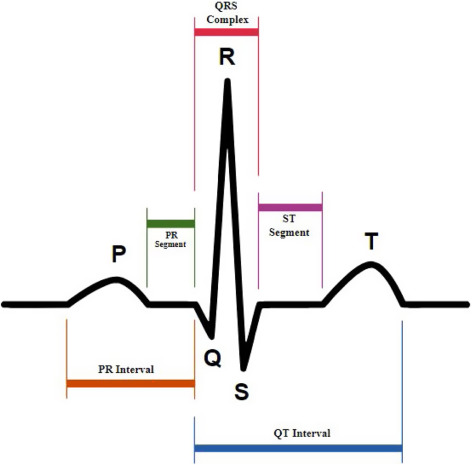
\includegraphics[width=0.7\linewidth,height=0.12\textheight,keepaspectratio]{images/LabelledHeartbeat.jpg}
    \caption[A single PQRST wave]{A single heartbeat with its main waves and intervals. Generated by the author from \cite{Mazomenos_ECG_2012}.}
    \label{fig:ecg-beat}
  \end{minipage}\hfill
  \begin{minipage}[b]{0.52\linewidth}
    \centering
    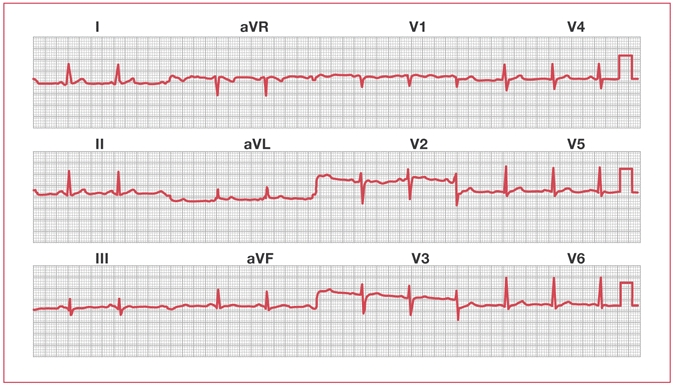
\includegraphics[width=0.7\linewidth,height=0.12\textheight,keepaspectratio]{images/ECGGrid.jpg}
    \caption[An ECG paper trace]{A twelve-lead ECG printed as a $3\times4$ grid of leads \cite{ashley_conquering_2004}.}
    \label{fig:ecg-grid}
  \end{minipage}
  \Description{Two images: a single labelled heartbeat showing the P wave, QRS complex, T wave and intervals, and a twelve-lead ECG printed as a three-by-four grid.}
\end{figure}

The target classes depend on the trace properties. For example, arrhythmias alter the rate or rhythm of the heart \cite{nhs_heart_2018}, like atrial fibrillation, which produces irregularly spaced beats without distinct P waves \cite{van_gelder_2024_2024}, whereas atrial flutter produces a regular saw-tooth pattern \cite{cosio_atrial_2017}. Bundle branch blocks widen the QRS complex \cite{scherbak_left_2024}, MI alters the ST segment and T wave, and hypertrophy changes the wave amplitude \cite{channer_myocardial_2002}. The diagnostic superclasses are therefore characterised principally by waveform \emph{morphology}, whereas the rhythm classes depend on \emph{timing}, which an image conveys only through its grid scale. The PTB-XL dataset annotates 21,800 twelve-lead recordings from approximately 19,000 patients with five diagnostic superclasses and rhythm statements, and permits several labels per record \cite{wagner_ptbxl_2020}, so the classification task is multi-label.

\subsubsection{ECG Digitisation Approach}
\label{sec:digitisation}
\label{sec:ecg-imaging}
Printed and photographed ECGs cannot be processed by software that expects digital signals \cite{shivashankara_ecg-image-kit_2024}. Paper records also exhibit creases, tears, faded ink, stains, shadows and skew \cite{physionet_challenge_2024}, and image resolution limits the precision with which timing can be measured. The PhysioNet Challenge 2024 invited teams to digitise and classify paper ECGs \cite{physionet_challenge_2024}, and its entries illustrate two distinct approaches.


Digitisation reconstructs the signal from the image by locating the grid, separating the leads and tracing each waveform, so that established signal-based classifiers can then be applied. The Challenge evaluated it by the SNR of the recovered signal \cite{physionet_challenge_2024}. Entries ranged from classical pipelines, which located each lead using binarisation, Gaussian smoothing and Canny edge detection \cite{hempel_driving_2024}, to other hybrid methods. The winning digitisation entry combined Hough-transform rotation correction with deep-learning segmentation of the trace and vectorisation of the result \cite{krones_combining_2024}. Its authors acknowledge, however, that the method assumed a common lead order, layout and grid scale, and that such models demand substantial data, time and computational resources \cite{krones_combining_2024}. Although digitisation yields measurable intervals, its stages are sequentially dependent, so an error in locating the grid propagates to every reconstructed lead.

\subsubsection{Direct Classification Approach}
\label{sec:direct-classification}

Direct classification instead predicts the diagnosis from the image itself. This removes the chain of dependent stages, but requires the model to infer timing from pixels, thus its performance depends on how the training images were produced. Two resources support this approach. ECG-Image-Kit renders synthetic images from real signals, with optional artefacts such as wrinkles and handwriting \cite{shivashankara_ecg-image-kit_2024}, and the ECG-Image-Database provides 35,595 images of 1,977 PTB-XL and Emory Healthcare records that were printed, degraded, and scanned or photographed \cite{reyna_ecg-image-database_2024}. A smaller collection of degraded real images is also available \cite{khan_ecg_2021}, although not used. Augmentation may narrow the gap between synthetic and real data: the winning digitisation team rendered at least four randomly augmented images of each PTB-XL record \cite{krones_combining_2024}, exposing the model to creases, rotation and noise during training. In view of the cost and layout assumptions of digitisation, the present work adopts direct classification, using timing measurements from a lighter detection stage (Section~\ref{sec:waveform}) only as supplementary features.

\subsection{Extracting Information from ECG Images}
\label{sec:extract-group}

Whichever approach is adopted, information must first be extracted from a degraded image.

\subsubsection{Pre-processing and Noise Removal}
\label{sec:preprocessing}

Preprocessing applies the methods of Section~\ref{sec:image-processing} to defects introduced by printing and capture, but ECG images present particular risks. The grid may confuse a classifier, yet it is the sole record of the time and voltage scales and must therefore be measured before it is removed. As the trace is only a few pixels wide, smoothing can erase P waves and QRS peaks, and rotation correction based on detected lines cannot completely reverse the perspective distortion of a photograph. Moreover, a CNN trained on sufficiently varied images may learn to tolerate these defects, in which case preprocessing offers little benefit. Consistent with \citet{barrett_foundations_2004}, preprocessing is accordingly evaluated by its effect on classification rather than by the visual quality of the image.

\subsubsection{Feature Extraction}
\label{sec:features}

Classical ECG analysis relied on hand-designed features, like interval durations and wave amplitudes, which were passed to a conventional classifier \cite{de_chazal_automatic_2004}. Such features have a clear clinical interpretation, and RR regularity directly distinguishes regular from irregular rhythms, but their reliability depends on the success of every preceding detection stage. A CNN instead learns features directly from pixels \cite{lecun_deep_2015}, avoiding this dependency at the cost of reduced interpretability and a greater need for labelled data. The two approaches (Figure~\ref{fig:feature-extraction}) are complementary: learned features suit the morphology-based superclasses, whereas measured timing features provide the rhythm classes with information that a CNN would otherwise have to infer from an uncertain grid scale.

\begin{figure}[!htbp]
  \centering
  \makebox[\linewidth][c]{\scalebox{0.85}{%
  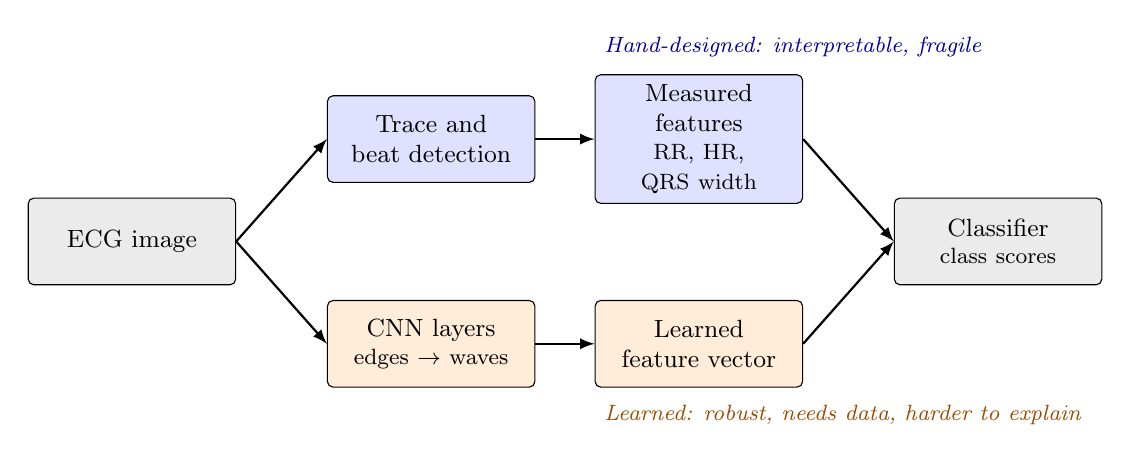
\begin{tikzpicture}[
      font=\small,
      box/.style={draw, rounded corners=2pt, align=center, minimum height=11mm,
                  text width=24mm, fill=#1},
      box/.default=white,
      arr/.style={-latex, thick}
    ]
    \node[box=black!8] (img) at (0,0) {ECG image};
    \node[box=blue!12] (det) at (38mm,13mm) {Trace and beat detection};
    \node[box=blue!12] (meas) at (72mm,13mm) {Measured features\\[-1pt]\footnotesize RR, HR, QRS width};
    \node[box=orange!15] (conv) at (38mm,-13mm) {CNN layers\\[-1pt]\footnotesize edges $\rightarrow$ waves};
    \node[box=orange!15] (learn) at (72mm,-13mm) {Learned feature vector};
    \node[box=black!8] (clf) at (110mm,0) {Classifier\\[-1pt]\footnotesize class scores};

    \draw[arr] (img.east) -- (det.west);
    \draw[arr] (det) -- (meas);
    \draw[arr] (meas.east) -- (clf.west);
    \draw[arr] (img.east) -- (conv.west);
    \draw[arr] (conv) -- (learn);
    \draw[arr] (learn.east) -- (clf.west);

    \node[anchor=south west, font=\footnotesize\itshape, text=blue!60!black]
      at ([yshift=1mm]meas.north west) {Hand-designed: interpretable, fragile};
    \node[anchor=north west, font=\footnotesize\itshape, text=orange!60!black]
      at ([yshift=-1mm]learn.south west) {Learned: robust, needs data, harder to explain};
  \end{tikzpicture}%
  }}
  \caption{Hand-designed and learned feature extraction from an ECG image. In the proposed system, timing features from detected beats are passed to the classifier alongside the features learned by the CNN.}
  \label{fig:feature-extraction}
  \Description{Hand-designed and learned feature extraction from an ECG image. This project
    will pass timing features from detected beats to the classifier alongside the features the CNN learns.}
\end{figure}

\subsubsection{Waveform Detection}
\label{sec:waveform}

In digital signals, waveform detection typically locates the QRS complex; the Pan--Tompkins algorithm band-pass filters, differentiates and squares the signal before applying adaptive thresholds \cite{pan_real-time_1985}. In images, the trace must first be isolated: published pipelines binarise the image, remove the grid and text, locate each lead with a Hough transform, and reduce each column of the trace to a single value before converting it to time and voltage \cite{wu_automated_2022}. On clean images, such methods can be accurate, achieving correlations of 0.94 \cite{randazzo_development_2022} and approximately 0.99 on standard layouts \cite{wu_automated_2022} against reference signals. The same studies, however, reveal their fragility. Correlation fell to approximately 0.96 on printed and rescanned ECGs, and images with overlapping leads had to be excluded \cite{wu_automated_2022}. Since a single missed or spurious peak alters every subsequent RR interval, detection will be evaluated on real images against Pan--Tompkins applied to the source signal, with the classifier reverting to the image alone if detection proves unreliable.

\subsection{Classification and Evaluation}
\label{sec:class-group}

This subsection reviews the classifiers applied to ECGs and the practices needed to evaluate them reliably.

\subsubsection{ECG Classification Algorithms}
\label{sec:ml-ecg}

Deep learning has largely superseded feature-based ECG classification. On signals, a CNN achieved cardiologist-level rhythm classification (F1 of 0.837 compared with 0.780 for cardiologists) \cite{hannun_cardiologist_2019}, whilst a network outperformed cardiology residents on six 12-lead abnormalities \cite{ribeiro_automatic_2020}in addition to a PTB-XL benchmark finding convolutional architectures, particularly ResNet- and Inception-based models, to perform best \cite{strodthoff_deep_2021}. These results demonstrate that the target classes are learnable, albeit from signals with a known scale.

Image-based classification is a more recent development. \citet{sangha_automated_2022} trained a CNN on images generated from signals and reported strong performance on external and printed ECGs. \citet{gliner_domain_2023} adapted a model from scanned to phone-captured images, and \citet{wang_pipeline_2025} fine-tuned a ConvNeXt backbone first on synthetic and then on external images. Owing to the scarcity of labelled ECG images, these studies rely on transfer learning from networks pretrained on natural images, such as ResNet \cite{he_deep_2016,yosinski_transfer_2014}. More recent architectures offer alternatives: Vision Transformers can outperform CNNs, but only when pretrained on very large datasets \cite{dosovitskiy_image_2021}, whereas ConvNeXt modernises the convolutional design and performs comparably to transformers at similar cost \cite{liu_convnet_2022}. Given the limited data and a single GPU, a compact CNN compared against a pretrained ResNet is the most feasible design, with architecture treated as an experimental variable. The principal signal and image-based studies are summarised in Table~\ref{tab:ecg-studies} (Appendix~\ref{app:lit}).

\subsubsection{ECG Dataset Evaluation}
\label{sec:ml-eval}

Four recurring weaknesses are evident in the evaluation of ECG classifiers. First, the classes are imbalanced, so accuracy may remain high even when rare conditions are missed. Sensitivity, specificity and MCC provide a more informative assessment \cite{chicco_advantages_2020}. Imbalance may also be mitigated during training by weighting the loss towards rare classes, oversampling them, or adopting focal loss, which down-weights easily classified examples \cite{lin_focal_2017}. Second, records must be partitioned by patient, as in PTB-XL's recommended folds \cite{wagner_ptbxl_2020}, to prevent the same patient appearing in both training and test sets - \citet{wang_pipeline_2025} acknowledge that their results might have been inflated by such leakage. Third, labels are imperfect: those in PTB-XL derive from at most two cardiologists \cite{wagner_ptbxl_2020}, and inter-rater agreement can be only poor to moderate \cite{dhutia_interrater_2017}, therfore a high AUROC partly reflects agreement with imperfect labels.

Fourth, performance may not generalise across patient groups. \citet{noseworthy_assessing_2020} observed that ECG characteristics vary by race without affecting their CNN's performance, and recommended that new ECG models report performance by ethnicity, race, age and sex. A comparison of 56 arrhythmia algorithms on over 130,000 ECGs found that performance varied with age, and that a fairness constraint reduced bias at a modest cost in performance \cite{perez_alday_age_2022}. As PTB-XL was recorded between 1989 and 1996 using a single manufacturer's devices \cite{wagner_ptbxl_2020}, generalisation to other populations cannot be assessed here and is acknowledged as a limitation.

\subsection{Trustworthy Outputs}
\label{sec:trust-group}

A decision-support system must also show how far its outputs can be trusted, and why they were produced.

\subsubsection{Calibration and Uncertainty}
\label{sec:calibration}

A model intended to support decisions must indicate the extent to which its outputs can be trusted. \citet{guo_calibration_2017} demonstrated that modern networks are frequently overconfident, and that temperature scaling, which divides the scores by a single parameter $T$ fitted on validation data, is a simple and effective solution. For multi-label outputs, each class score $z_k$ becomes $\hat{p}_k = \sigma(z_k/T)$; as division by $T$ preserves the ranking of scores, AUROC is unaffected, and only the reliability of the probabilities (measured by the ECE), changes. Its application to independent sigmoid outputs is, however, an adaptation of the original single-label formulation.

Several alternatives exist. One example is Platt scaling, which fits a logistic function to the scores \cite{platt_probabilistic_1999}. Training with focal loss yields better-calibrated networks and, combined with temperature scaling, achieved state-of-the-art calibration \cite{mukhoti_calibrating_2020}. Deep ensembles \cite{lakshminarayanan_simple_2017} and Monte Carlo dropout \cite{gal_dropout_2016} provide fuller estimates of uncertainty and improved calibration in signal-based atrial fibrillation detection \cite{chen_quantifying_2022}, although ensembles multiply the training cost. The literature is divided on whether calibration persists under distribution shift: \citet{ovadia_trust_2019} found that it deteriorates as data diverge from the training distribution, whereas \citet{minderer_revisiting_2021} found that recent architectures remain well calibrated and identified architecture as a major factor. The present work addresses precisely this question, since $T$ is fitted on rendered images but applied to real ones. Whether calibration survives this shift is therefore measured rather than assumed.

\subsubsection{Explainability and Presentation to Users}
\label{sec:explainability}

Grad-CAM produces a heatmap of the image regions that most influenced a CNN's prediction for a given class \cite{selvaraju_gradcam_2017}. Being class-specific and computationally inexpensive, it allows a heatmap to be displayed for each flagged condition. Model-agnostic alternatives such as LIME \cite{ribeiro_why_2016} and SHAP \cite{lundberg_unified_2017} explain predictions by perturbing the input, but are considerably slower on large images and attribute importance to pixels rather than to individual waves.

All such methods are subject to criticism. \citet{adebayo_sanity_2018} found that certain saliency maps changed little when a model's weights were randomised, indicating that a plausible heatmap need not reflect what the model has learned. \citet{ghassemi_false_2021} extends this argument, contending that current explainability methods are unlikely to provide trust or transparency for individual patient decisions, and that rigorous validation offers a more direct route to those goals. Explanations are, moreover, seldom evaluated. A review of explainable AI in cardiology found that 43\% of studies did not evaluate their explanations, and only 11\% involved clinicians \cite{salih_review_2024}.

User requirements also vary with expertise. Clinicians seek explanations that help them judge when a model can be trusted \cite{tonekaboni_what_2019}. In interviews with 23 clinicians, accuracy was valued above explanation, and visualisations of what the algorithm had analysed were preferred \cite{hughes-noehrer_contrasting_2024}, while an experiment with 44 cardiologists found that explanations increased the trust of novices more than that of experts, and were sometimes misinterpreted \cite{cabitza_painting_2023}. Accordingly, heatmaps in this work will be validated against known cases rather than accepted at face value, and separate views will be provided for a range of users, evaluated through a user study and the System Usability Scale \cite{brooke_sus_1996,bangor_empirical_2008}.

\subsection{Existing Systems and Limitations}
\label{sec:existing-systems}

Most ECGs are interpreted by software on the recording device, but its accuracy is limited. Its output requires over-reading by an experienced clinician. It may also be accepted uncritically by inexperienced users, and it cannot be obtained from printouts \cite{schlapfer_computer-interpreted_2017}. Table~\ref{tab:existing-systems} compares the principal deep-learning systems.

\begin{table}[H]
  \centering
  \footnotesize
  \renewcommand{\arraystretch}{1.0}
  \caption{Comparison of existing ECG analysis systems and the planned system.}
  \label{tab:existing-systems}
  \begin{tabular}{@{}p{0.17\linewidth} p{0.17\linewidth} p{0.27\linewidth} p{0.31\linewidth}@{}}
    \toprule
    \textbf{System} & \textbf{Input} & \textbf{Key features} & \textbf{Limitations} \\
    \midrule
    \citet{sangha_automated_2022} &
      Images generated from signals &
      CNN tested on held-out, external and printed ECGs (AUROC 0.98) &
      Trained on generated images; reports discrimination only, not calibration \\
    \citet{gliner_domain_2023} &
      Scans; phone-captured frames &
      Domain adaptation from scans to phone images (AUROC 0.91) &
      Phone images made by filming printed pages; six unseen formats tested \\
    \citet{wang_pipeline_2025} &
      Synthetic and external scanned images &
      Challenge-winning ConvNeXt pipeline (AUROC about 0.97) &
      Evaluated on synthetic PTB-XL images, with possible leakage \\
    \citet{krones_combining_2024} &
      Scanned and photographed images &
      Winning digitisation: Hough transform and deep-learning segmentation &
      Assumes a fixed layout and grid scale; resource-intensive \\
    \midrule
    This project (planned) &
      Rendered images for training; real images for testing &
      CNN with timing features; calibration; Grad-CAM; user views; user study &
      Labels from at most two annotators; real test set limited to the ECG-Image-Database \\
    \bottomrule
  \end{tabular}
\end{table}

Four gaps therefore remain. First, image-based classification has been evaluated largely on synthetic or limited real images, and the strongest results may be inflated by leakage. Second, calibration has been studied for signals \cite{chen_quantifying_2022}, whereas image-based studies report discrimination alone. Third, explanations are rarely evaluated \cite{salih_review_2024}, despite substantial evidence that they can mislead \cite{adebayo_sanity_2018,ghassemi_false_2021}. Fourth, the presentation of results to users of differing expertise has not been investigated for image-based ECG tools or for non-expert users.

\subsection{Summary}
\label{sec:lit-summary}

Whereas signal-based deep learning for ECG analysis is well established, image-based work has relied on synthetic data and has paid limited attention to whether its confidence can be trusted or its explanations understood. Table~\ref{tab:lit-decisions} summarises how the literature reviewed in this section informs the design of the proposed system.

\begin{table}[!htbp]
  \centering
  \footnotesize
  \renewcommand{\arraystretch}{1.0}
  \caption{Design decisions, the alternatives considered, and the literature behind each choice.}
  \label{tab:lit-decisions}
  \begin{tabular}{@{}p{0.14\linewidth} p{0.22\linewidth} p{0.24\linewidth} p{0.31\linewidth}@{}}
    \toprule
    \textbf{Decision} & \textbf{Choice} & \textbf{Alternatives} & \textbf{Reason} \\
    \midrule
    Approach & Direct classification, with timing features & Full digitisation \cite{krones_combining_2024} & Avoids chained errors and fixed-layout assumptions (Section~\ref{sec:ecg-imaging}) \\
    Training data & Rendered PTB-XL images, tested on real images & Real images only & Real labelled images are too few to train on \cite{reyna_ecg-image-database_2024} \\
    Model & Own CNN vs pretrained ResNet & ConvNeXt, Vision Transformer \cite{liu_convnet_2022,dosovitskiy_image_2021} & Transformers need very large pretraining; limited data and one GPU \\
    Imbalance & Class-weighted loss; per-class thresholds & Oversampling, focal loss \cite{lin_focal_2017} & Simple and widely used; focal loss kept as an option \\
    Calibration & Temperature scaling & Platt scaling, ensembles, MC dropout \cite{platt_probabilistic_1999,lakshminarayanan_simple_2017,gal_dropout_2016} & One parameter, AUROC unchanged; ensembles too costly \cite{guo_calibration_2017} \\
    Explanation & Grad-CAM, checked on known cases & LIME, SHAP \cite{ribeiro_why_2016,lundberg_unified_2017} & Class-specific and fast; checking addresses \cite{adebayo_sanity_2018,ghassemi_false_2021} \\
    Presentation & User and clinical views, user study with SUS & Single interface & Novices and experts respond differently \cite{cabitza_painting_2023,tonekaboni_what_2019} \\
    \bottomrule
  \end{tabular}
\end{table}

% Methodology
%%%%%%%%%%%%%%%%%%%%
\section{Methodology}
\label{ch:method}

\subsection{Research Goals}
\label{sec:goals}
The project addresses one main question:
\begin{quote}
\emph{Can a CNN trained on rendered ECG images detect cardiac abnormalities and rhythm disorders in real ECG images, and how can its information be made reliable and understandable to users?}
\end{quote}
It is divided into three sub-questions, each tied to a gap from Section~\ref{ch:lit} and to the objectives in brackets:
\begin{itemize}
  \item \textbf{SQ1 (Obj 1--Obj 4):} How much does performance fall from rendered to real images, and how far do preprocessing and timing features reduce the fall?
  \item \textbf{SQ2 (Obj 5):} How reliable is the model's confidence per class, and how much does temperature scaling improve it?
  \item \textbf{SQ3 (Obj 6):} Do the explanations highlight the expected regions, and can users understand the confidence and explanation shown?
\end{itemize}

\subsection{Project Requirements}
\label{sec:requirements}
Table~\ref{tab:functional-req} lists the requirements in order of development, prioritised with MoSCoW to limit scope creep. Requirements with a planned fallback are rated Should rather than Must, and each requirement has a test (Section~\ref{sec:testing}).

\begingroup
\footnotesize
\setlength{\arrayrulewidth}{0.8pt}
\renewcommand{\arraystretch}{1.0}
\begin{longtable}{|p{0.08\linewidth}|p{0.60\linewidth}|p{0.105\linewidth}|p{0.085\linewidth}|}
  \caption{Functional and non-functional requirements.}
  \label{tab:functional-req} \\
    \hline
    \rowcolor{cyan!90!black}
    \textcolor{white}{\textbf{ID}} & \textcolor{white}{\textbf{Requirement}} &
    \textcolor{white}{\textbf{MoSCoW}} & \textcolor{white}{\textbf{Obj.}} \\
    \hline
  \endfirsthead
    \hline
    \rowcolor{cyan!90!black}
    \textcolor{white}{\textbf{ID}} & \textcolor{white}{\textbf{Requirement}} &
    \textcolor{white}{\textbf{MoSCoW}} & \textcolor{white}{\textbf{Obj.}} \\
    \hline
  \endhead
    FR01 & The user can upload an ECG image (scan or photograph). & Must & Obj 1, Obj 6 \\
    \hline
    FR02 & The system preprocesses the image. & Must & Obj 2 \\
    \hline
    FR03 & The system detects the trace and locates the R peaks. & Should & Obj 2 \\
    \hline
    FR04 & The system extracts the HR and RR regularity. & Should & Obj 2 \\
    \hline
    FR05 & The system flags possible abnormalities for the five diagnostic superclasses. & Must & Obj 3 \\
    \hline
    FR06 & The system flags the four rhythm classes. & Should & Obj 3 \\
    \hline
    FR07 & Each flag shows a calibrated confidence score. & Must & Obj 5 \\
    \hline
    FR08 & A heatmap is overlaid on the original image for each flagged class. & Should & Obj 6 \\
    \hline
    FR09 & The interface shows the measured values (HR and RR intervals). & Should & Obj 2, Obj 6 \\
    \hline
    FR10 & A plain-language explanation is shown for each flagged condition (User View). & Should & Obj 6 \\
    \hline
    FR11 & A labelled diagram of the waves is available for reference. & Could & Obj 6 \\
    \hline
    FR12 & A clinical view shows all nine classes and their thresholds, and fuller values to measure. & Could & Obj 6 \\
    \hline
    FR13 & The user can export a result. & Could & Obj 6 \\
    \hline
    FR14 & The user can save a result. & Could & Obj 6 \\
    \hline
    FR15 & The system warns the user if an image is too poor in quality to analyse. & Should & Obj 2 \\
    \hline
    FR16 & Real-time/live ECG analysis. & Won't & N/A \\ % as no equipment
    \hline
    FR17 & Advice on treatments, or diagnosis. & Won't & N/A \\
    \hline
    NFR01 & The system returns a result within 10\,s of upload on the development PC. & Must & Obj 6 \\
    \hline
    NFR02 & Mean AUROC across the five superclasses on the rendered test fold is at least 0.85. & Must & Obj 3 \\
    \hline
    NFR03 & After temperature scaling, the ECE is at most 0.05 for each reported class, and lower than before scaling. & Must & Obj 5 \\
    \hline
    NFR04 & The fall in AUROC from rendered to real images is measured per class, with a target of at most 0.10 for the five superclasses. & Should & Obj 4 \\
    \hline
    NFR05 & Without training, at least 70\% of study participants correctly interpret the confidence and heatmap, and the mean SUS score is at least 68. & Should & Obj 6 \\
    \hline
    NFR06 & The results screen shows the model's limitations, such as classes with few real test images. & Should & Obj 6 \\
    \hline
    NFR07 & Uploaded images are not shared or stored beyond the session. & Should & N/A \\
    \hline
    NFR08 & Results can be reproduced from the repository (fixed seeds, pinned package versions, scripts for the reported tables). & Must & Obj 3 \\
    \hline
    NFR09 & The trained system runs on a standard laptop without a GPU (training excluded). & Could & N/A \\
    \hline
    NFR10 & The pipeline, model and interface are separate modules, so one can be replaced without changing the others. & Could & N/A \\
    \hline
\end{longtable}
\endgroup

\subsection{Project Development Process}
\label{sec:dev-plan}

The work is divided into seven phases (Figure~\ref{fig:workflow}). Phases overlap wherever one does not need the other's output, for example the GUI is built while the model trains (Appendix~\ref{app:gantt}).

\begin{figure}[!htbp]
  \centering
  \makebox[\linewidth][c]{\scalebox{0.8}{%
  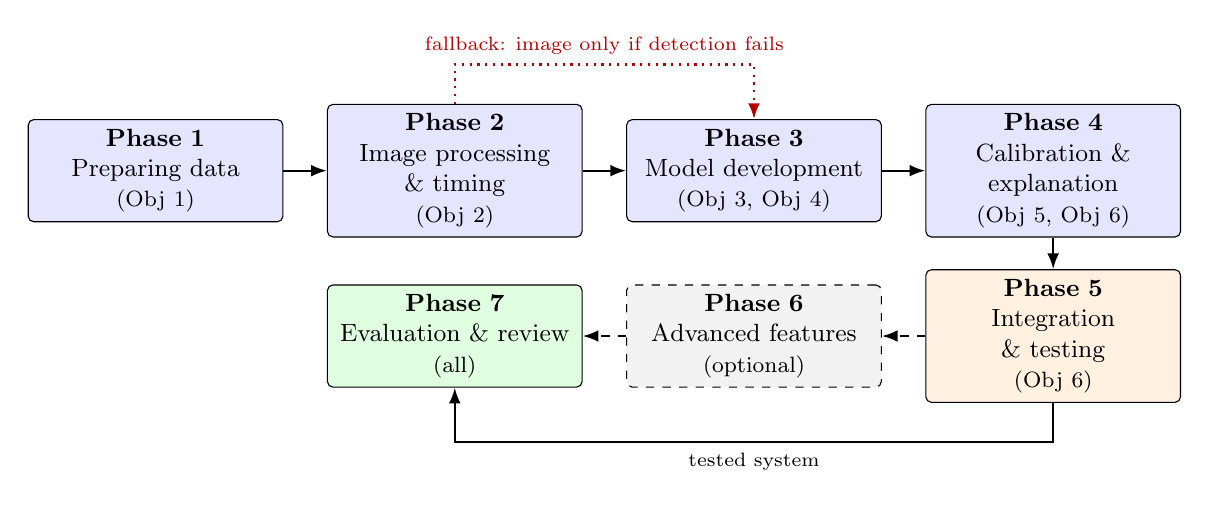
\begin{tikzpicture}[
      font=\small,
      phase/.style={draw, rounded corners=2pt, align=center, text width=30mm,
                    minimum height=11mm, fill=#1},
      phase/.default=blue!10,
      arr/.style={-{Latex[length=2mm]}, thick}
    ]
    \node[phase] (p1) at (0,0)     {\textbf{Phase 1}\\Preparing data\\\footnotesize(Obj 1)};
    \node[phase] (p2) at (38mm,0)  {\textbf{Phase 2}\\Image processing\\\& timing\\\footnotesize(Obj 2)};
    \node[phase] (p3) at (76mm,0)  {\textbf{Phase 3}\\Model development\\\footnotesize(Obj 3, Obj 4)};
    \node[phase] (p4) at (114mm,0) {\textbf{Phase 4}\\Calibration \& explanation\\\footnotesize(Obj 5, Obj 6)};
    \node[phase=orange!12] (p5) at (114mm,-21mm) {\textbf{Phase 5}\\Integration \& testing\\\footnotesize(Obj 6)};
    \node[phase=black!5, dashed] (p6) at (76mm,-21mm) {\textbf{Phase 6}\\Advanced features\\\footnotesize(optional)};
    \node[phase=green!12] (p7) at (38mm,-21mm) {\textbf{Phase 7}\\Evaluation \& review\\\footnotesize(all)};

    \draw[arr] (p1) -- (p2);
    \draw[arr] (p2) -- (p3);
    \draw[arr] (p3) -- (p4);
    \draw[arr] (p4) -- (p5);
    \draw[arr, dashed] (p5) -- (p6);
    \draw[arr, dashed] (p6) -- (p7);
    \draw[arr] (p5.south) -- ++(0,-5mm) -| node[pos=0.25, below, font=\scriptsize]{tested system} (p7.south);

    % fallback
    \draw[arr, dotted, red!70!black] (p2.north) -- ++(0,5mm) -| node[pos=0.25, above, font=\scriptsize]{fallback: image only if detection fails} (p3.north);
  \end{tikzpicture}%
  }}
  \caption{Project workflow. Phase 6 is optional and is dropped first if the schedule slips.}
  \label{fig:workflow}
  \Description{Project workflow. Phase 6 is optional and is dropped first if the schedule slips.}
\end{figure}

\textbf{Phase 1: Preparing data (Obj 1).} Training images will be rendered from PTB-XL with ECG-Image-Kit, labelled with the nine classes and split by patient. A real test set will be prepared from the PTB-XL part of the ECG-Image-Database, and its patients excluded from the training folds to prevent leakage.

\textbf{Phase 2: Image processing and timing (Obj 2).} OpenCV will isolate the trace; R peaks, heart rate and RR regularity will then be measured and checked against Pan--Tompkins on the source signal. A quality check will warn when the trace cannot be found (FR15).

\textbf{Phase 3: Model development (Obj 3, Obj 4).} A multi-label CNN will be trained on rendered images with a class-weighted loss, with and without timing features, and a pretrained ResNet fine-tuned on the same splits for comparison.

\textbf{Phase 4: Calibration and explanation (Obj 5, Obj 6).} Temperature scaling will be fitted on the validation fold, and Grad-CAM heatmaps checked against expected regions and for shortcuts such as attention on the grid or text.

\textbf{Phases 5--7: Integration, extensions and evaluation (Obj 6).} The modules will be combined into one Python application and tested against the requirements; if time is short, the interface will be reduced to uploading, flagging and the heatmap. The project will then be evaluated (Section~\ref{sec:eval}), including the user study under the approved ethics application, with an expert review as the fallback. The risks behind these fallbacks are in Table~\ref{tab:risks} (Appendix~\ref{app:risks}).



\subsection{Testing and Evaluation Strategy}
\label{sec:evaluation}

Testing will verify each requirement; evaluation will assess the project against its aims and research questions. Limitations are in Section~\ref{sec:ml-eval} and Appendix~\ref{app:ples}.

\subsubsection{Testing}
\label{sec:testing}

Each module will be tested on its own before the integrated system. The Requirements Traceability Matrix (Tables~\ref{tab:rtm-fr} and~\ref{tab:rtm-nfr}, Appendix~\ref{app:rtm}) maps every requirement to its module, deliverable and test case, and will record whether it was met. A detected R peak counts as correct if within $\pm200$\,ms of Pan--Tompkins on the source signal \cite{pan_real-time_1985}.

\subsubsection{Evaluation}
\label{sec:eval}

Each objective will be marked as achieved, partly achieved or not achieved using the evidence mapped in Table~\ref{tab:obj-eval} (Appendix~\ref{app:rtm}), the percentage achieved will be reported, and any shortfalls will be explained.

\textbf{Experiments.} Models will be tested on the rendered PTB-XL test fold (folds 1--8 train, 9 validation, 10 test) \cite{wagner_ptbxl_2020} and on real ECG-Image-Database images \cite{reyna_ecg-image-database_2024}. Class thresholds will be chosen on the validation fold to maximise MCC (0.5 for classes with too few cases) and held fixed, and each class scored by sensitivity, specificity, MCC and AUROC \cite{chicco_advantages_2020}. The rendered-to-real gap (SQ1) is the per-class difference in AUROC and MCC. Calibration (SQ2) will be measured per class by the ECE before and after temperature scaling, with reliability diagrams. The own CNN will be compared with the pretrained model and a variant without timing features, with bootstrap confidence intervals for small classes. For SQ3, heatmaps will be checked on labelled cases, and students will complete a comprehension questionnaire and the SUS \cite{brooke_sus_1996}.

\textbf{Success criteria} are the targets of FR03, FR04 and NFR02--NFR05; the rendered-to-real gap is reported either way.

% Feasibility
%%%%%%%%%%%%%%%%%%%%
\section{Feasibility}
\label{ch:feasibility}

This section shows that the plan in Section~\ref{ch:method} is achievable, through the datasets, the system design and the prototypes built so far.

\subsection{Datasets}
\label{sec:datasets}

PTB-XL provides 21,800 labelled twelve-lead ECGs with patient-wise folds \cite{wagner_ptbxl_2020}. The classes are imbalanced, from 9,514 normal records to only 73 with atrial flutter; the counts for all nine classes are in Table~\ref{tab:class-counts} (Appendix~\ref{app:lit}). The ECG-Image-Database provides 35,595 real images of 1,977 recordings, 977 from PTB-XL and 1,000 from Emory Healthcare \cite{reyna_ecg-image-database_2024}. The PTB-XL part can be matched to PTB-XL labels by record, giving the labelled real test set; the real images per class, and whether the Emory labels map to the nine classes, will be checked in Phase 1. Their patients will be removed from the training folds to prevent leakage, and rare classes may only be evaluated on rendered images.

\subsection{Design}
\label{sec:design}

The system will be developed in Python, using OpenCV \cite{bradski_opencv_2000} for image processing, PyTorch for the networks and Grad-CAM, and PySide6 integrated with matplotlib for the interface, chosen for their mature libraries. Training will run on my own PC, which has a GPU, with the code on GitHub (Appendix~\ref{app:repo}). Figure~\ref{fig:architecture} shows the architecture, with each module's inputs and outputs. The modules are separate, so any one can be replaced (NFR10). The GUI offers a user view with explanations and a clinical view with every class score and threshold.

\begin{figure}[H]
  \centering
  \makebox[\linewidth][c]{\scalebox{0.85}{%
  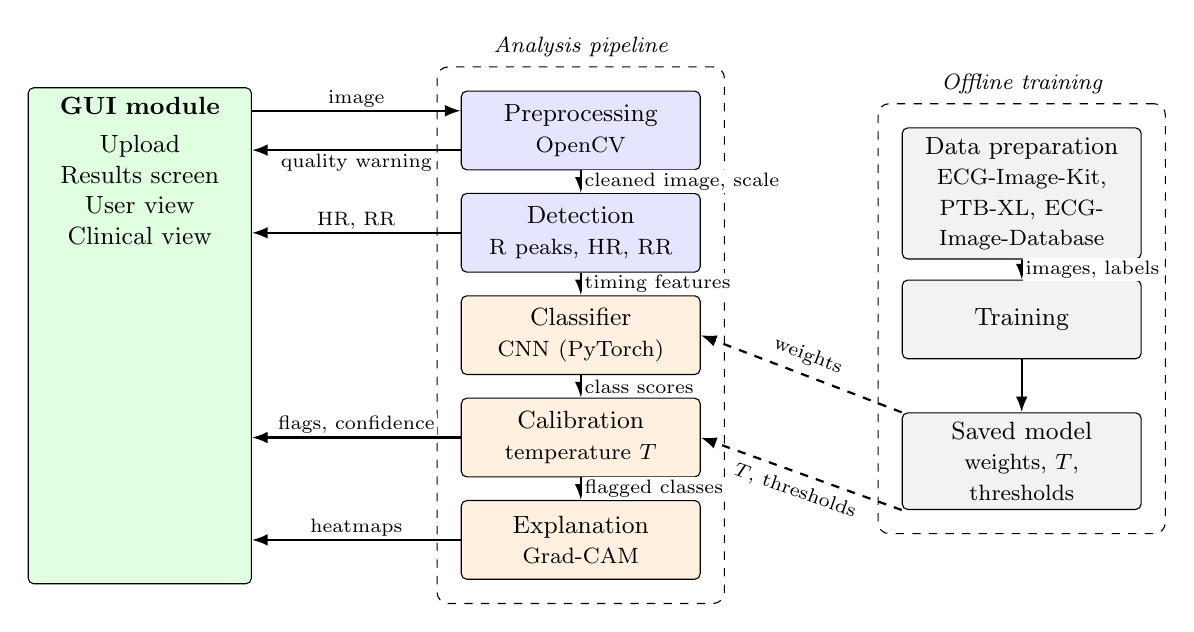
\begin{tikzpicture}[
      font=\small,
      mod/.style={draw, rounded corners=2pt, align=center, text width=28mm,
                  minimum height=10mm, fill=#1},
      mod/.default=blue!10,
      arr/.style={-{Latex[length=2mm]}, thick},
      lab/.style={font=\scriptsize, fill=white, inner sep=1pt}
    ]
    % analysis pipeline (middle column)
    \node[mod] (pre) at (0,0)      {Preprocessing\\\footnotesize OpenCV};
    \node[mod] (det) at (0,-13mm)  {Detection\\\footnotesize R peaks, HR, RR};
    \node[mod=orange!12] (clf) at (0,-26mm) {Classifier\\\footnotesize CNN (PyTorch)};
    \node[mod=orange!12] (cal) at (0,-39mm) {Calibration\\\footnotesize temperature $T$};
    \node[mod=orange!12] (exp) at (0,-52mm) {Explanation\\\footnotesize Grad-CAM};
    \node[draw, dashed, rounded corners, inner sep=3mm, fit=(pre)(exp),
          label={[font=\footnotesize\itshape]above:Analysis pipeline}] (pipe) {};

    % GUI (left)
    \node[mod=green!12, minimum height=63mm, text width=26mm, anchor=north]
         (gui) at (-56mm,5.5mm) {};
    \node[align=center, font=\small, text width=24mm, anchor=north] at (gui.north)
         {\textbf{GUI module}\\[3pt]Upload\\Results screen\\User view\\Clinical view};

    % offline training (right)
    \node[mod=black!5] (data) at (56mm,-8mm) {Data preparation\\\footnotesize ECG-Image-Kit, PTB-XL, ECG-Image-Database};
    \node[mod=black!5] (train) at (56mm,-24mm) {Training};
    \node[mod=black!5] (store) at (56mm,-42mm) {Saved model\\\footnotesize weights, $T$, thresholds};
    \node[draw, dashed, rounded corners, inner sep=3mm, fit=(data)(store),
          label={[font=\footnotesize\itshape]above:Offline training}] {};

    % pipeline flow
    \draw[arr] (pre) -- node[lab, right]{cleaned image, scale} (det);
    \draw[arr] (det) -- node[lab, right]{timing features} (clf);
    \draw[arr] (clf) -- node[lab, right]{class scores} (cal);
    \draw[arr] (cal) -- node[lab, right]{flagged classes} (exp);

    % GUI <-> pipeline
    \draw[arr] (gui.east |- 0,2.5mm) -- node[lab, above]{image} ([yshift=2.5mm]pre.west);
    \draw[arr] ([yshift=-2.5mm]pre.west) -- node[lab, below]{quality warning} (gui.east |- 0,-2.5mm);
    \draw[arr] (det.west) -- node[lab, above]{HR, RR} (gui.east |- det);
    \draw[arr] (cal.west) -- node[lab, above]{flags, confidence} (gui.east |- cal);
    \draw[arr] (exp.west) -- node[lab, above]{heatmaps} (gui.east |- exp);

    % offline flow
    \draw[arr] (data) -- node[lab, right]{images, labels} (train);
    \draw[arr] (train) -- (store);
    \draw[arr, dashed] (store.north west) -- node[font=\scriptsize, above, sloped, pos=0.5]{weights} (clf.east);
    \draw[arr, dashed] (store.south west) -- node[font=\scriptsize, below, sloped, pos=0.5]{$T$, thresholds} (cal.east);
  \end{tikzpicture}%
  }}
  \caption{Planned system architecture and processing pipeline, showing the modules, their inputs and outputs, and how they connect.}
  \label{fig:architecture}
  \Description{Planned system architecture and processing pipeline, showing the modules, their inputs and outputs, and how they connect.}
\end{figure}

\subsection{Prototypes}
\label{sec:prototypes}

Three prototypes test the main risks (Table~\ref{tab:prototypes}); Figures~\ref{fig:rendered} and~\ref{fig:proto2} show the first two, and the wireframes are in Appendix~\ref{app:wireframes}.

\begin{table}[H]
  \centering
  \footnotesize
  \setlength{\arrayrulewidth}{0.8pt}
  \renewcommand{\arraystretch}{1.15}
  \caption{Prototypes and their results.} % CHANGED: "Status" column replaced by "Result" to give measurable feasibility evidence
  \label{tab:prototypes}
  % TODO: replace each [ADD: ...] with your own measured figure (do not leave any in the final PDF)
  \begin{tabular}{|p{0.18\linewidth}|p{0.38\linewidth}|p{0.34\linewidth}|}
    \hline
    \rowcolor{cyan!90!black}
    \textcolor{white}{\textbf{Prototype}} & \textcolor{white}{\textbf{Demonstrates}} &
    \textcolor{white}{\textbf{Result}} \\
    \hline
    1: Data and rendering & Labels mapped to nine classes; records rendered with ECG-Image-Kit. & \textbf{3 out of 3 signal records were rendered}. \\
    \hline
    2: Preprocessing & Thresholding and feature detection remove colour and grid, leaving the trace. & \textbf{Traces were isolated in 3 of 3 test images}. \\
    \hline
    3: GUI wireframes & Layout of the user and clinical views. & \textbf{Both views designed and mapped to FR07--FR12 (Appendix~\ref{app:wireframes})}. \\ % CHECK: confirm your wireframes show FR07--FR12
    \hline
  \end{tabular}
\end{table}

\begin{figure}[H]
  \centering
  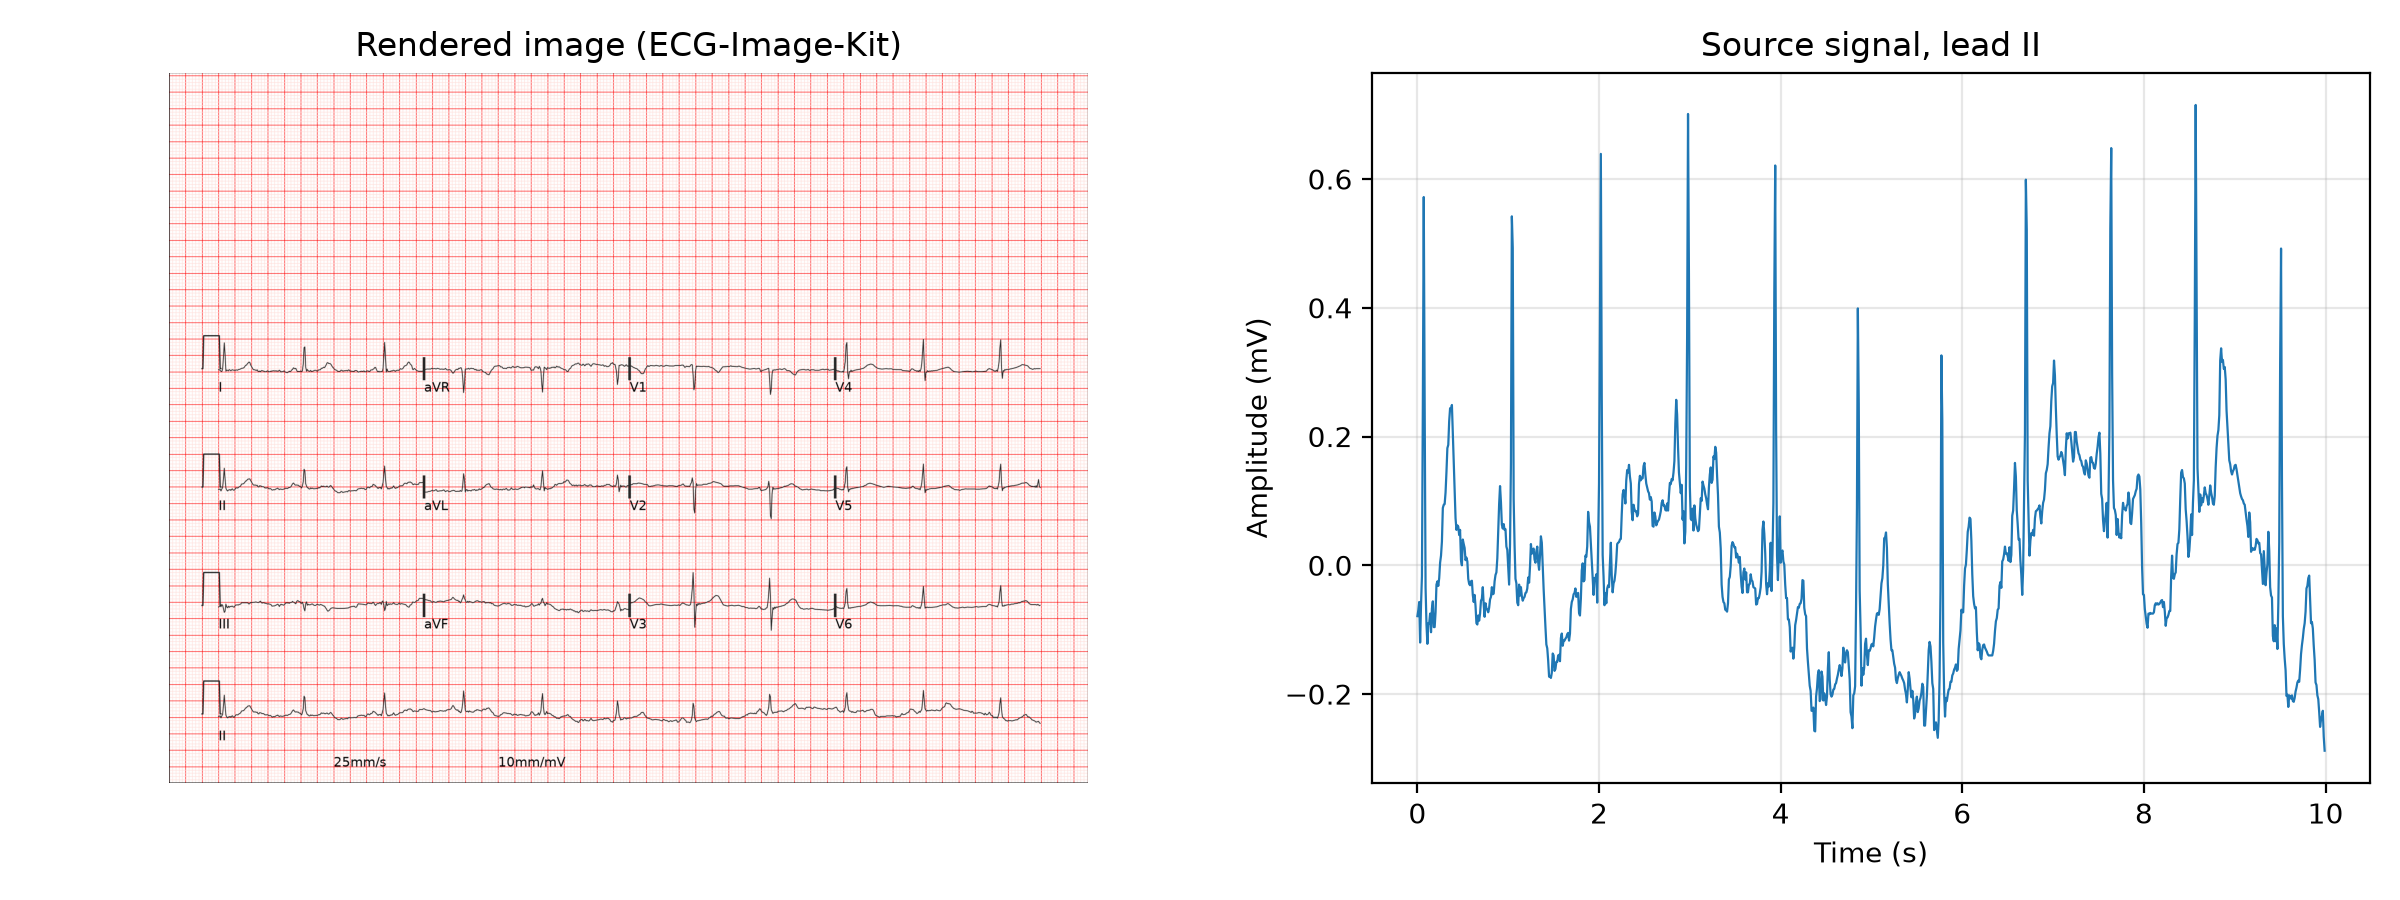
\includegraphics[width=0.85\linewidth,height=0.13\textheight,keepaspectratio]{images/rendered_vs_signal.png}
  \caption{Prototype 1: PTB-XL record 00001\_lr rendered with ECG-Image-Kit
    \cite{shivashankara_ecg-image-kit_2024} (left), and the lead II signal it was generated
    from (right). Both show 11 beats at about 0.9--1.0\,s spacing.}
  \label{fig:rendered}
  \Description{Prototype 1: PTB-XL record 00001_lr rendered with ECG-Image-Kit
     (left), and the lead II signal it was generated
    from (right). Both show 11 beats at about 0.9--1.0,s spacing.}
\end{figure}

\begin{figure}[H]
  \centering
  \begin{subfigure}[b]{0.24\linewidth}
    \centering
    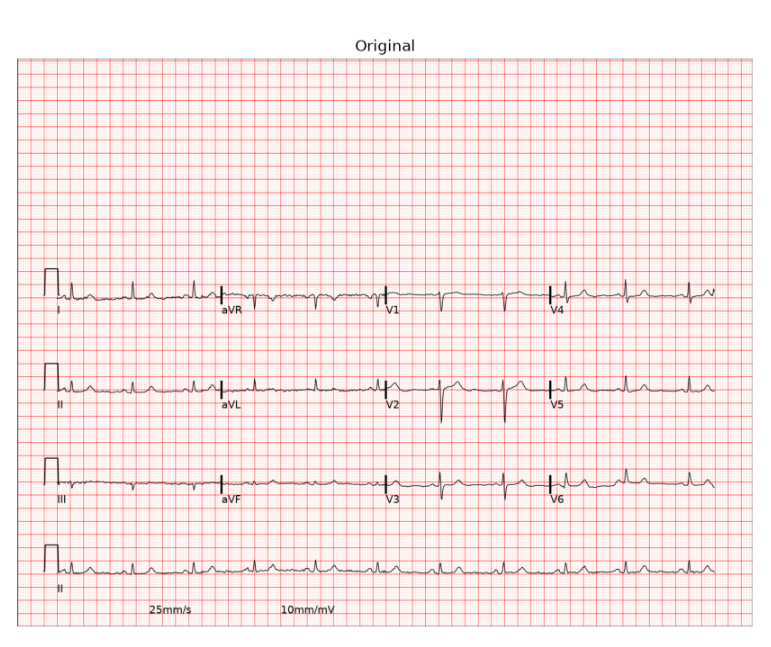
\includegraphics[width=\linewidth]{images/p2_initial.png}
    \caption{Initial Image.}
    \label{fig:img1}
  \end{subfigure}\hfill
  \begin{subfigure}[b]{0.24\linewidth}
    \centering
    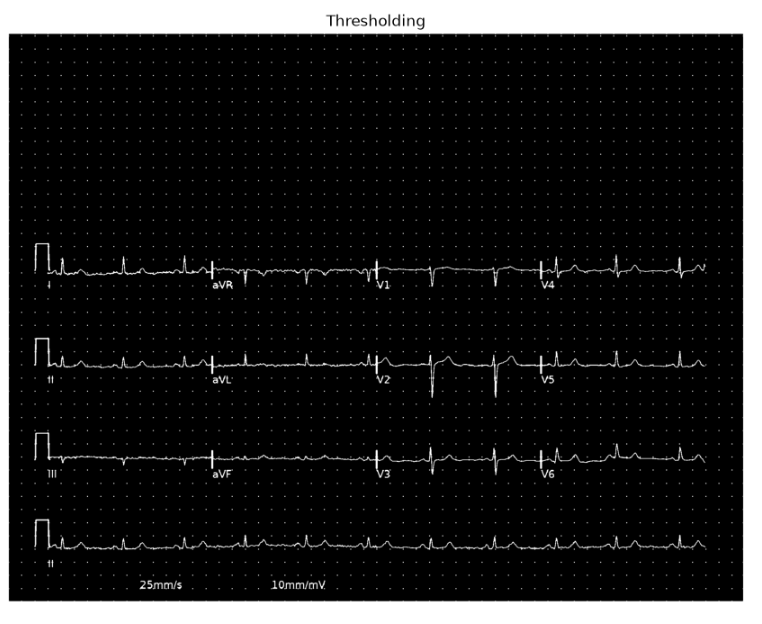
\includegraphics[width=\linewidth]{images/p2_thre.png}
    \caption{Image thresholded.}
    \label{fig:img2}
  \end{subfigure}\hfill
  \begin{subfigure}[b]{0.24\linewidth}
    \centering
    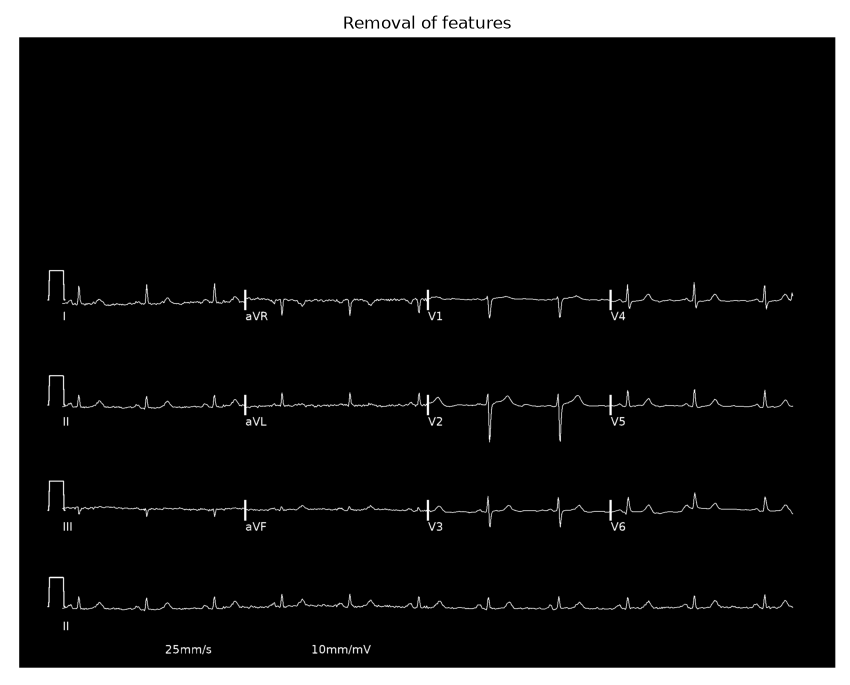
\includegraphics[width=\linewidth]{images/p2_remov.png}
    \caption{Features Removed.}
    \label{fig:img3}
  \end{subfigure}
  \caption{Extracting a waveform from an ECG.}
  \label{fig:proto2}
  \Description{Initial Image.}
\end{figure}
\subsection{Risks}
\label{sec:feas-risks}

The full risk assessment is in Table~\ref{tab:risks} (Appendix~\ref{app:risks}). The main feasibility risks are the rendered-to-real gap (R1), detection failing on poor images (R2), rare classes (R3) and time for the full interface (R10); their fallbacks are reporting the gap, classifying from the image alone, reporting class counts, and a reduced interface.

% Conclusion
%%%%%%%%%%%%%%%%%%%%
\section{Conclusion}
\label{ch:conc}

\subsection{Summary}
\label{sec:conc-summary}

This project will build and evaluate a CNN application that flags possible abnormalities in ECG images, reports calibrated confidence, and explains its predictions to different users. It addresses four gaps: limited testing on real images, missing calibration, unevaluated explanations, and little evidence on presenting results to different users.

The work is organised into seven phases (Section~\ref{sec:dev-plan}), tested through the Requirements Traceability Matrix and evaluated against the objectives. All three prototypes are complete.

\subsection{Expected Contributions}
\label{sec:contributions}

\begin{enumerate}\setlength{\itemsep}{0pt}\setlength{\parskip}{0pt}
  \item \textbf{A per-class measure of the rendered-to-real gap.} Testing on real images of the same recordings, with leakage removed, will show which classes transfer and whether timing features help (SQ1).
  \item \textbf{Calibration under data shift for a multi-label image classifier.} Per-class calibration error on rendered and real images will show whether confidence fitted on rendered images can be trusted on real ones (SQ2).
  \item \textbf{Evidence on presenting results to non-expert users.} The user study will show whether students can interpret calibrated confidence and heatmaps (SQ3).
\end{enumerate}

\subsection{Next Steps}
\label{sec:next-steps}
 Semester 2 will follow the Gantt schedule (Figure~\ref{fig:gantt-s2}) in Appendix~\ref{app:gantt}. The first weeks will prepare the data and build detection, which every later phase depends on; CNN training will follow, with the GUI developed in parallel, aiming for a working prototype by week 9. The user study and evaluation follow in weeks 9--11; if the schedule slips, the fallbacks in Section~\ref{sec:dev-plan} apply.

%%%%%%%%%%%%%%%%%%%%%%%%%%%%%%%%%%%%%%%%%%%%%%%%%%
% BACK MATTER
%%%%%%%%%%%%%%%%%%%%%%%%%%%%%%%%%%%%%%%%%%%%%%%%%%

% References
% list of references

\newpage
\renewcommand{\bibname}{References} % change name to References
% \phantomsection
% \addcontentsline{toc}{section}{References}
\bibliography{references}
% \bibliographystyle{plainnat}

% using Harvard style
% \bibliographystyle{agsm}

% using ACM style (defined in acm_settings.tex)
\bibliographystyle{ACM-Reference-Format}

% using APA style (requires apacite package)
% \bibliographystyle{apacite}

% Appendices
\newpage
\appendix

\crefalias{chapter}{appendixchapter} % for appendix crossreferences
\raggedbottom % ADDED: stops large blank gaps around the Gantt charts when a float moves to the next page

\section{Project Management}
\label{app:pm}

\subsection{Gantt Chart}
\label{app:gantt}

Figures~\ref{fig:gantt-s1} and~\ref{fig:gantt-s2} show the schedule for both semesters. Tasks overlap where they can run in parallel, and the fallbacks in Section~\ref{sec:dev-plan} allow the plan to be reduced if it slips.

\begin{figure}[H]
  \centering
  % CHANGED (supervisor feedback): tasks now overlap instead of running one
  % after another like a waterfall. Arrows are kept only for real
  % dependencies (a task that genuinely cannot start until another ends).
  % CHECK: adjust the weeks so they match what you actually did in Semester 1.
  \resizebox{\linewidth}{!}{%
  \begin{ganttchart}[
      hgrid,
      vgrid={*1{black!25, dotted}},
      x unit=1.0cm,
      y unit title=0.8cm,
      y unit chart=0.75cm,
      time slot format=simple,
      title label font=\normalsize\bfseries,
      bar label font=\normalsize,
      group label font=\normalsize\bfseries,
      milestone label font=\normalsize\itshape,
      bar height=0.55,
      bar/.append style={fill=blue!30},
      group/.append style={fill=black!70},
      milestone/.append style={fill=red!60},
      link/.style={-latex, thick, black!60}
    ]{1}{12}

    \gantttitle{Week}{12} \\
    \gantttitlelist{1,...,12}{1} \\

    \ganttgroup{D1 report}{1}{11} \\
    \ganttbar[name=supervisor]{Supervisor selection}{1}{2} \\
    \ganttbar[name=topic]{Topic selection}{1}{3} \\
    \ganttbar[name=ethics]{Ethics form}{3}{7} \\
    \ganttbar[name=lit]{Literature review}{3}{9} \\
    \ganttbar[name=intro]{Introduction}{3}{6} \\
    \ganttbar[name=meth]{Methodology}{6}{9} \\
    \ganttbar[name=req]{Requirements}{7}{9} \\
    \ganttbar[name=prt]{Prototypes}{8}{11} \\
    \ganttbar[name=pp]{Project plan}{8}{10} \\
    \ganttbar[name=feasi]{Feasibility}{9}{11} \\
    \ganttbar[name=appe]{Appendices}{6}{11} \\
    \ganttbar[name=abs]{Abstract and conclusion}{10}{11} \\
    \ganttmilestone[name=esub]{Ethics submission}{7} \\
    \ganttmilestone[name=dsub]{D1 submission}{11}

    \ganttlink{topic}{ethics}
    \ganttlink{ethics}{esub}
    \ganttlink{abs}{dsub}
  \end{ganttchart}%
  }
  \Description{Gantt chart for Semester 1 showing overlapping report tasks over 12 weeks, with the ethics submission in week 7 and the D1 submission in week 11.}
  \caption{Project plan for Semester 1. Overlapping bars show tasks carried out in parallel; arrows show tasks that depend on another finishing first.}
  \label{fig:gantt-s1}
\end{figure}

\begin{figure}[H]
  \centering
  % CHANGED (supervisor feedback): implementation tasks now overlap, e.g. GUI
  % development runs alongside model training, and writing runs throughout.
  % Arrows mark only real dependencies.
  \resizebox{\linewidth}{!}{%
  \begin{ganttchart}[
      hgrid,
      vgrid={*1{black!25, dotted}},
      x unit=1.0cm,
      y unit title=0.8cm,
      y unit chart=0.75cm,
      time slot format=simple,
      title label font=\normalsize\bfseries,
      bar label font=\normalsize,
      group label font=\normalsize\bfseries,
      milestone label font=\normalsize\itshape,
      bar height=0.55,
      bar/.append style={fill=blue!30},
      group/.append style={fill=black!70},
      milestone/.append style={fill=red!60},
      link/.style={-latex, thick, black!60}
    ]{1}{12}

    \gantttitle{Week}{12} \\
    \gantttitlelist{1,...,12}{1} \\

    \ganttgroup{Implementation and evaluation}{1}{11} \\
    \ganttbar[name=env]{Environment setup}{1}{1} \\
    \ganttbar[name=img]{Image generation}{1}{3} \\
    \ganttbar[name=pre]{Preprocessing and detection}{2}{5} \\
    \ganttbar[name=cnn]{CNN creation}{3}{4} \\
    \ganttbar[name=train]{CNN training}{4}{7} \\
    \ganttbar[name=pt]{Pretrained comparison}{5}{7} \\
    \ganttbar[name=cal]{Calibration}{8}{8} \\
    \ganttbar[name=heat]{Heatmaps and explanations}{8}{9} \\
    \ganttbar[name=gui]{GUI development}{3}{9} \\
    \ganttbar[name=int]{Integration and testing}{8}{10} \\
    \ganttmilestone[name=proto]{Working prototype}{9} \\
    \ganttbar[name=study]{User study}{9}{11} \\
    \ganttbar[name=eval]{Evaluation and results}{9}{11} \\
    \ganttbar[name=write]{Dissertation writing}{4}{11} \\
    \ganttmilestone[name=final]{Final submission}{11}

    \ganttlink{env}{pre}
    \ganttlink{img}{train}
    \ganttlink{train}{cal}
    \ganttlink{cal}{proto}
    \ganttlink{gui}{proto}
    \ganttlink{write}{final}
  \end{ganttchart}%
  }
  \Description{Gantt chart for Semester 2 showing overlapping implementation tasks, a working prototype in week 9, and the final submission in week 11.}
  \caption{Project plan for Semester 2. GUI development runs alongside model training, and writing runs throughout.}
  \label{fig:gantt-s2}
\end{figure}

\subsection{Risk Assessment and Mitigation}
\label{app:risks}

Table~\ref{tab:risks} gives the full risk assessment. Each risk is rated once for its likelihood and its severity, and lists every mitigation planned for it. Section~\ref{sec:feas-risks} refers to the risks most relevant to feasibility by their IDs.

\begingroup
\footnotesize
\renewcommand{\arraystretch}{1.2}
\begin{longtable}{|p{0.05\linewidth}|p{0.24\linewidth}|p{0.11\linewidth}|p{0.10\linewidth}|p{0.35\linewidth}|}
  \caption{Risk assessment and mitigation.}
  \label{tab:risks} \\
    \hline
    \textbf{ID} & \textbf{Risk} & \textbf{Likelihood} & \textbf{Severity} & \textbf{Mitigation} \\
    \hline
  \endfirsthead
    \multicolumn{5}{l}{\footnotesize\itshape Table~\ref{tab:risks} continued} \\
    \hline
    \textbf{ID} & \textbf{Risk} & \textbf{Likelihood} & \textbf{Severity} & \textbf{Mitigation} \\
    \hline
  \endhead
    \multicolumn{5}{|l|}{\textbf{Technical risks}} \\
    \hline
    R1 & A model trained on rendered images may not work on real images. & \High & \High &
      Generate a large training set with ECG-Image-Kit, and add augmentation that imitates real artefacts. Evaluate on real images and report the gap as a result. \\
    \hline
    R2 & Trace detection fails on poor-quality real images. & \Med & \Med &
      Evaluate detection separately on real images. If it is too unreliable, the CNN uses the image alone, and the failure is reported. \\
    \hline
    R3 & Some classes have too few examples to train a model. & \High & \Med &
      Report results per class with counts and bootstrap confidence intervals. Rare classes such as atrial flutter may be combined with atrial fibrillation, or evaluated on rendered images only. \\
    \hline
    R4 & Class imbalance biases the model towards the majority class. & \High & \Med &
      Use class weights to balance the loss function, and imbalance-aware metrics (sensitivity, specificity, MCC, AUROC). Choose a threshold for each class on the validation fold. \\
    \hline
    R5 & The ECG-Image-Database has very few images for some classes. & \High & \Med &
      Evaluate only the classes with enough real images; report the rest as a limitation. \\
    \hline
    R6 & Labels are subjective and may be inconsistent. & \Med & \Med &
      Use the PTB-XL validation and test folds, whose labels were checked to a higher standard, and report label quality as a limitation. \\
    \hline
    R7 & Heatmaps may be misleading. & \Med & \Med &
      Check heatmaps against known cases and for shortcuts; mask the grid if needed; evaluate the heatmaps in the user study. \\
    \hline
    R8 & The CNN underperforms. & \Med & \Med &
      Fine-tune a pretrained model on the same splits for comparison, and use it as the main model if it performs better. \\
    \hline
    R9 & Training is too slow. & \Low & \Low &
      Use smaller models or a lower image resolution to reduce the cost. \\
    \hline
    \multicolumn{5}{|l|}{\textbf{Project and ethical risks}} \\
    \hline
    R10 & The scope is too large for the time available, including the full interface. & \Med & \Med &
      Prioritise requirements with MoSCoW so that the most important are implemented first. Reduce the interface to uploading, flagging and the heatmap if time is short. \\
    \hline
    R11 & There are not enough participants for the user study. & \Med & \Med &
      Start recruitment early. If this fails, an expert review replaces the study. \\
    \hline
    R12 & Clinicians are not able to take part. & \High & \Low &
      Base the requirements on published studies of clinicians. State the limitation, and describe clinician testing as future work. \\
    \hline
    R13 & Software problems, such as package conflicts. & \Med & \Low &
      Use version control, and a virtual environment with a recorded list of package versions. \\
    \hline
    R14 & Loss of code or data. & \Low & \High &
      Keep remote copies on GitHub and regular backups of results (Section~\ref{app:repo}). \\
    \hline
    R15 & The user study goes beyond its approved ethical scope. & \Low & \High &
      Keep the study within the approved scope. Process images locally, and destroy participant data on completion of the project. \\
    \hline
    R16 & A dataset or tool update changes its availability or licence. & \Low & \Low &
      Keep local copies of the datasets; check and cite their licences. \\
    \hline
    R17 & The author cannot complete the project due to illness or other personal reasons. & \Low & \High &
      Plan the project with deadlines, and keep the supervisor informed of progress. \\
    \hline
\end{longtable}
\endgroup

\subsubsection{Professional Issues}
The project follows the BCS Code of Conduct, of which the following principles apply most directly:
\begin{itemize}\setlength{\itemsep}{0pt}\setlength{\parskip}{0pt}
  \item \textbf{Public interest.} Results will be reported honestly, including those that do not support the project's aims, and preliminary results will be presented as pilot results.
  \item \textbf{Professional competence and integrity.} All datasets, tools and publications are cited, and the use of generative AI is declared in the Declaration of Authorship. % CHANGED: the template puts the GenAI statement in the declaration form
  \item \textbf{Duty to the profession.} All code is kept under version control, and the environment and data sources are documented so that results can be reproduced (NFR08).
\end{itemize}

\subsubsection{Legal Issues}
ECG recordings are health data, which the UK GDPR and the Data Protection Act 2018 treat as special category personal data \cite{dpa_2018}. The training and test data are drawn from public, de-identified datasets, so the project processes no identifiable patient records. User-study responses are pseudonymised during collection, fully anonymised before analysis, held on university-approved storage, and deleted at the end of the project. Images uploaded to the interface are processed locally and are not retained beyond the session (NFR07).

Software intended to support the diagnosis of a medical condition may be regulated as a medical device under the UK Medical Devices Regulations 2002 \cite{uk_mdr_2002}, and the MHRA advises that this depends on the software's stated intended purpose \cite{mhra_samd_2025}. The present system is an academic prototype with a stated non-diagnostic purpose (FR17); it will not be placed on the market or used in patient care. Any future clinical use would require regulatory approval, a clinical safety assessment, and validation on considerably more data than this project uses.
PTB-XL and the ECG-Image-Database are distributed under the Creative Commons Attribution 4.0 licence, and ECG-Image-Kit under the BSD 3-Clause licence; each is cited wherever it is used, and images generated with the toolkit are used under these terms. Figures from other sources are reproduced with citation, and figures produced by the author are identified as such. Copyright in the code and the report is held in accordance with the university's regulations.

\subsubsection{Ethical Issues}
The project has received ethical approval on the 20/11/2026. Participants in the user study will give informed consent, may withdraw at any time, and will not be asked for personal health information.
The principal ethical risk of a tool that flags abnormalities is inappropriate reliance on its output. A false negative may give unwarranted reassurance, and a false positive may cause unnecessary anxiety. Automation bias is documented for computer-interpreted ECGs, whose output may be accepted uncritically by inexperienced users \cite{schlapfer_computer-interpreted_2017}, and explanations have been found to raise the trust of novices more than that of experts \cite{cabitza_painting_2023}. The system therefore reports a calibrated confidence for each class so that uncertainty is visible, validates its heatmaps against known cases, states its limitations on the results screen (NFR06), and presents itself as a learning and research aid whose output must be checked by a qualified person.

\subsubsection{Social Issues}
PTB-XL was recorded between 1989 and 1996 using a single manufacturer's devices \cite{wagner_ptbxl_2020}, and ECG-based models have shown differences in performance across age, sex and ethnicity \cite{noseworthy_assessing_2020,perez_alday_age_2022}. As the project cannot test generalisation to other populations, it makes no claim that its results would hold elsewhere, and reports results by age and sex where the data permit.

Systems that read ECG images could support teaching and extend automated analysis to settings where only paper records exist. Conversely, over-reliance on such a tool could reduce learning, so the interface explains its reasoning in plain language and is designed to be accessible to users with differing needs. Finally, training deep networks consumes considerable energy; the project limits this by using a compact model and, where appropriate, pretrained weights.

\subsection{Repository Management}
\label{app:repo}

The project's code will be kept in a private GitHub repository, with a working copy on the development PC. The repository will be organised by module, matching the architecture in Section~\ref{sec:design}: separate folders for data preparation scripts, preprocessing, detection, models, calibration and explanation, the GUI, experiment configurations, and tests.

\textbf{Data and large files.} The datasets (PTB-XL and the ECG-Image-Database) and the rendered images are too large to store in Git, and are distributed under their own licences, so they will be excluded with a \texttt{.gitignore} file. The repository will instead contain the scripts that download the datasets and render the images, so that they can be recreated (NFR08). Trained model weights will also be stored outside Git.

\textbf{Branching and commits.} The \texttt{main} branch will always hold a working version. New work will be done on a separate branch for each phase or feature, and merged into \texttt{main} once its tests pass. Commits will be small, with descriptive messages, and each milestone (D1, the working prototype and the final submission) will be tagged so that it can be recovered.

\textbf{Reproducibility.} The Python environment will be recorded in a \texttt{requirements.txt} file with pinned package versions, and each experiment will have a configuration file recording its settings and random seed, so that the reported results can be regenerated from a fresh clone (NFR08, TC23).

\textbf{Backups.} GitHub will act as the remote copy of the code. Results, model weights and the report will be backed up weekly to the university OneDrive (R14).




\section{Wireframes}
\label{app:wireframes}

\begin{figure}[H]
  \centering
  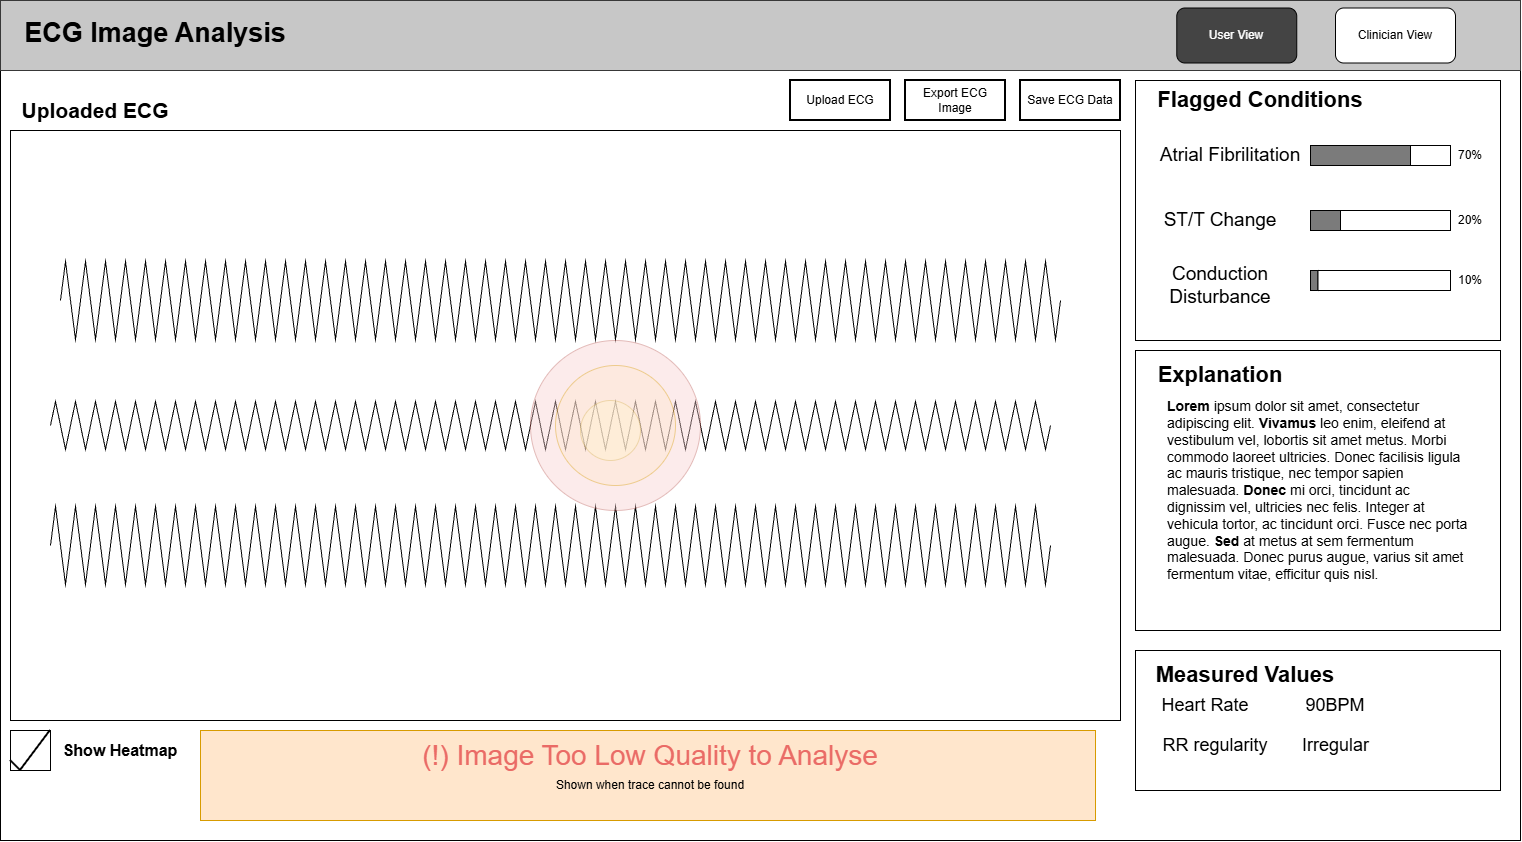
\includegraphics[width=0.85\linewidth,height=0.5\textheight,keepaspectratio]{images/user_view.png}
  \caption{Prototype 3: Wireframe created of the user view.}
  \label{fig:proto3user}
  \Description{Prototype 3: Wireframe created of the user view.}
\end{figure}

\begin{figure}[H]
  \centering
  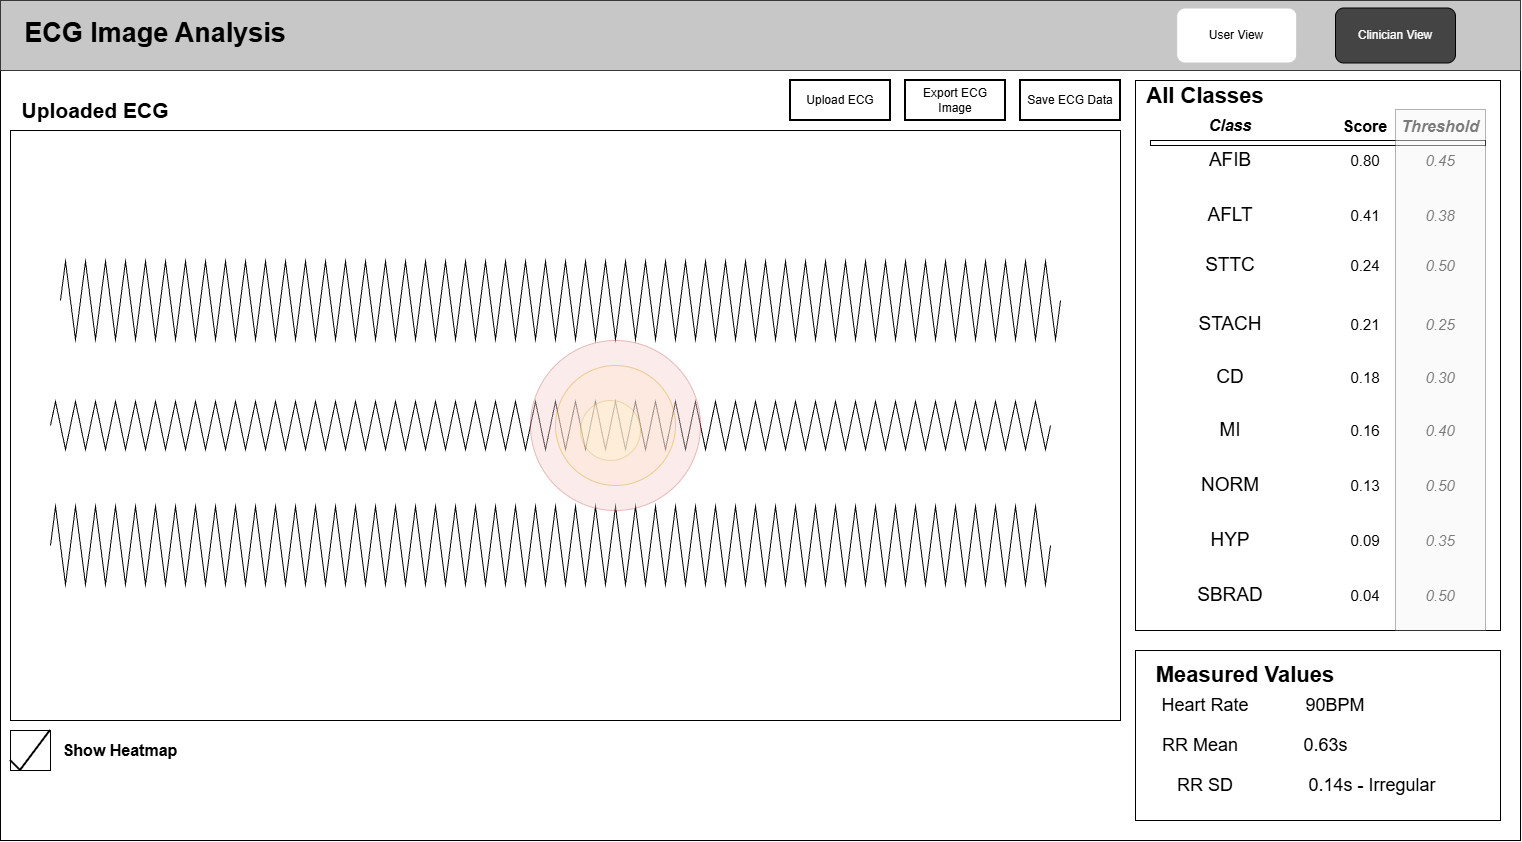
\includegraphics[width=0.85\linewidth,height=0.5\textheight,keepaspectratio]{images/clinician_view.png}
  \caption{Prototype 3: Wireframe created of the clinician view.}
  \label{fig:proto3clin}
  \Description{Prototype 3: Wireframe created of the clinician view.}
\end{figure}



\section{Requirements Traceability Matrix}
\label{app:rtm}

Tables~\ref{tab:rtm-fr} and~\ref{tab:rtm-nfr} map each requirement in Table~\ref{tab:functional-req} to the module that implements it, its deliverable and its test case. The result column will be completed after system testing. The Won't requirements (FR16 and FR17) are not implemented, so they are not tested.

\begin{table}[H]
  \centering
  \footnotesize
  \setlength{\arrayrulewidth}{0.8pt}
  \renewcommand{\arraystretch}{1.25}
  \caption{Requirements Traceability Matrix: functional requirements.}
  \label{tab:rtm-fr}
  \begin{tabular}{|p{0.07\linewidth}|p{0.15\linewidth}|p{0.16\linewidth}|p{0.39\linewidth}|p{0.08\linewidth}|}
    \hline
    \rowcolor{cyan!90!black}
    \textcolor{white}{\textbf{ID}} & \textcolor{white}{\textbf{Module}} &
    \textcolor{white}{\textbf{Deliverable}} & \textcolor{white}{\textbf{Test case}} &
    \textcolor{white}{\textbf{Result}} \\
    \hline
    FR01 & GUI & Upload screen & TC01: Upload a scan and a photograph (PNG and JPG); both load and are displayed. & \\
    \hline
    FR02 & Preprocessing & Preprocessing module & TC02: Run on 20 rendered and 20 real images; the output keeps the trace, removes the grid and records the grid scale. & \\
    \hline
    FR03 & Detection & R-peak detector & TC03: On images with a source signal, at least 90\% of R peaks are found within $\pm200$\,ms of Pan--Tompkins. & \\
    \hline
    FR04 & Detection & Timing features & TC04: Heart-rate mean absolute error is at most 5\,bpm against the source signal. & \\
    \hline
    FR05 & Classifier & Trained CNN & TC05: A score is produced for each of the five superclasses on the test fold (performance tested by TC17). & \\
    \hline
    FR06 & Classifier & Trained CNN & TC06: A score is produced for each rhythm class; performance is reported where class counts allow. & \\
    \hline
    FR07 & Calibration, GUI & Results screen & TC07: Each flag shows a probability between 0 and 1, taken after temperature scaling. & \\
    \hline
    FR08 & Explanation, GUI & Heatmap overlay & TC08: A heatmap aligned with the image is shown for each flagged class. & \\
    \hline
    FR09 & GUI & Results screen & TC09: The HR and RR values shown match the detector output. & \\
    \hline
    FR10 & GUI & Explanation text & TC10: Each of the nine classes shows its plain-language description when flagged. & \\
    \hline
    FR11 & GUI & Wave diagram & TC11: The labelled diagram opens from the results screen. & \\
    \hline
    FR12 & GUI & Clinical view & TC12: Switching view shows all nine scores with their thresholds, RR variability, and no teaching text. & \\
    \hline
    FR13 & GUI & Export function & TC13: The exported file opens and contains the flags and scores. & \\
    \hline
    FR14 & GUI & Save function & TC14: A saved result reloads with the same contents. & \\
    \hline
    FR15 & Preprocessing, Detection & Quality check & TC15: On 20 heavily degraded images a warning is shown and no flags are given; on 20 clean images no warning is shown. & \\
    \hline
  \end{tabular}
\end{table}

\begin{table}[H]
  \centering
  \footnotesize
  \setlength{\arrayrulewidth}{0.8pt}
  \renewcommand{\arraystretch}{1.25}
  \caption{Requirements Traceability Matrix: non-functional requirements.}
  \label{tab:rtm-nfr}
  \begin{tabular}{|p{0.07\linewidth}|p{0.15\linewidth}|p{0.16\linewidth}|p{0.39\linewidth}|p{0.08\linewidth}|}
    \hline
    \rowcolor{cyan!90!black}
    \textcolor{white}{\textbf{ID}} & \textcolor{white}{\textbf{Module}} &
    \textcolor{white}{\textbf{Deliverable}} & \textcolor{white}{\textbf{Test case}} &
    \textcolor{white}{\textbf{Result}} \\
    \hline
    NFR01 & Whole system & Integrated application & TC16: The time from upload to results is under 10\,s for each of 20 images on the development PC. & \\
    \hline
    NFR02 & Classifier & Evaluation report & TC17: Mean AUROC on PTB-XL fold 10 is at least 0.85 across the five superclasses. & \\
    \hline
    NFR03 & Calibration & Reliability diagrams & TC18: ECE is at most 0.05 for each reported class after scaling, and lower than before. & \\
    \hline
    NFR04 & Classifier & Rendered-to-real report & TC19: The fall in AUROC per class is at most 0.10 for the five superclasses. & \\
    \hline
    NFR05 & GUI & User-study results & TC20: At least 70\% of participants interpret the confidence and heatmap correctly; mean SUS is at least 68. & \\
    \hline
    NFR06 & GUI & Limitations panel & TC21: The results screen lists the classes with few or no real test images. & \\
    \hline
    NFR07 & GUI & Session handling & TC22: After the session closes, no uploaded image remains on disk. & \\
    \hline
    NFR08 & Repository & Scripts and environment file & TC23: Re-running the evaluation script from a fresh clone reproduces the reported metrics. & \\
    \hline
    NFR09 & Whole system & Integrated application & TC24: Inference runs on a laptop without a GPU. & \\
    \hline
    NFR10 & Architecture & Module interfaces & TC25: The own CNN is replaced with the pretrained model without changing the pipeline or GUI code. & \\
    \hline
  \end{tabular}
\end{table}

\begin{table}[H]
  \centering
  \footnotesize
  \setlength{\arrayrulewidth}{0.8pt}
  \renewcommand{\arraystretch}{1.12}
  \caption{Evidence used to evaluate each objective.}
  \label{tab:obj-eval}
  \begin{tabular}{|p{0.07\linewidth}|p{0.36\linewidth}|p{0.34\linewidth}|p{0.11\linewidth}|}
    \hline
    \rowcolor{cyan!90!black}
    \textcolor{white}{\textbf{Obj.}} & \textcolor{white}{\textbf{Evidence}} &
    \textcolor{white}{\textbf{Requirements and tests}} & \textcolor{white}{\textbf{Status}} \\
    \hline
    Obj 1 & Rendered training set and labelled real test set, with class counts & FR01; Phase 1 outputs & \\
    \hline
    Obj 2 & Preprocessing and detection results on rendered and real images & FR02--FR04, FR15; TC02--TC04, TC15 & \\
    \hline
    Obj 3 & Per-class sensitivity, specificity, MCC and AUROC & FR05, FR06, NFR02, NFR08; TC05, TC06, TC17, TC23 & \\
    \hline
    Obj 4 & Rendered-to-real gap per class & NFR04; TC19 & \\
    \hline
    Obj 5 & ECE and reliability diagrams before and after scaling & FR07, NFR03; TC07, TC18 & \\
    \hline
    Obj 6 & Heatmap checks, working GUI and user-study results & FR08--FR14, NFR01, NFR05, NFR06; TC08--TC16, TC20, TC21 & \\
    \hline
  \end{tabular}
\end{table}


\section{Supplementary Literature Material}
\label{app:lit}

\begin{table}[H]
  \centering
  \footnotesize
  \renewcommand{\arraystretch}{1.0}
  \caption{Image processing techniques relevant to ECG images, and their trade-offs.}
  \label{tab:techniques}
  \begin{tabular}{@{}p{0.27\linewidth} p{0.30\linewidth} p{0.37\linewidth}@{}}
    \toprule
    \textbf{Technique} & \textbf{Use} & \textbf{Trade-off} \\
    \midrule
    HE; CLAHE \cite{pizer_adaptive_1987,zuiderveld_contrast_1994} & Global; local contrast and uneven lighting & HE loses local detail; CLAHE needs tuning and can raise noise \\
    Gaussian and median filters \cite{gonzalez_digital_2018} & Random and salt-and-pepper noise & Blur edges and flatten thin peaks \\
    Bilateral filter; non-local means \cite{tomasi_bilateral_1998,verma_ali_2013,buades_non-local_2005} & Smooth flat regions while keeping edges & Slower; need tuning \\
    Notch filter (Fourier domain) \cite{gonzalez_digital_2018} & Removes regular patterns such as the grid & Struggles with faded or monochrome prints \\
    Homomorphic filter \cite{stockham_image_1972} & Suppresses illumination $i$, boosts reflectance $r$ & Can amplify noise \\
    Wavelet transform \cite{lepcha_deep_2023} & Multi-scale noise removal & Choice of scale and threshold \\
    Otsu thresholding \cite{otsu_threshold_1979}; edge detection \cite{canny_computational_1986} & Separate trace from background; find boundaries & Fail under uneven lighting; sensitive to noise \\
    \bottomrule
  \end{tabular}
\end{table}

\begin{table}[H]
  \centering
  \footnotesize
  \caption{Key studies in deep learning for ECG classification.}
  \label{tab:ecg-studies}
  \begin{tabular}{@{}p{0.13\linewidth} p{0.27\linewidth} p{0.25\linewidth} p{0.25\linewidth}@{}}
    \toprule
    \textbf{Study} & \textbf{Input and data} & \textbf{Reported result} &
      \textbf{Limitation for this project} \\
    \midrule
    \citet{hannun_cardiologist_2019} &
      Single-lead signals; 91,232 ECGs, 53,549 patients &
      12 rhythm classes; F1 0.837 vs.\ 0.780 for cardiologists &
      Single lead; signals, not images \\
    \citet{ribeiro_automatic_2020} &
      12-lead signals; over two million exams &
      Six abnormalities; F1 above 80\%, specificity above 99\% &
      Signals, not images \\
    \citet{strodthoff_deep_2021} &
      12-lead signals, PTB-XL &
      Convolutional models performed best &
      Signals; hidden weakness in subclasses \\
    \citet{sangha_automated_2022} &
      Images generated from signals; printed ECGs to test &
      Strong performance on held-out, external and printed ECGs (0.98 AUROC average) &
      Training images are generated from signals \\
    \citet{gliner_domain_2023} &
      79,226 scanned labelled ECGs plus unlabelled phone-captured frames &
      Average AUROC of 0.91 on phone-captured images &
      Phone images made by filming printed pages; six unseen formats tested \\
    \citet{wang_pipeline_2025} &
      Synthetic PTB-XL images plus external scanned sets &
      AUROC about 0.97 on the hidden test set &
      Synthetic test data; possible leakage from PTB-XL \\
    \bottomrule
  \end{tabular}
\end{table}

\begin{table}[H]
  \centering
  \footnotesize
      \caption{Records per class in PTB-XL.}
    \label{tab:class-counts}
    \begin{tabular}{@{}lr@{}}
      \toprule
      \textbf{Class} & \textbf{Records} \\
      \midrule
      Normal & 9514 \\
      Myocardial infarction & 5469 \\
      ST/T change & 5235 \\
      Conduction disturbance & 4898 \\
      Hypertrophy & 2649 \\
      Atrial fibrillation & 1514 \\
      Atrial flutter & 73 \\
      Sinus tachycardia & 826 \\
      Sinus bradycardia & 637 \\
      \bottomrule
    \end{tabular}
\end{table}

\begin{figure}[H]
  \centering
  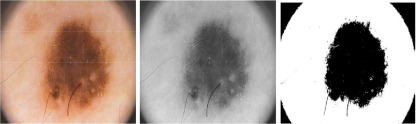
\includegraphics[width=0.38\linewidth]{images/OtsuSegmentation.jpg}
  \caption[Otsu segmentation of a dermatoscopic image]{Example of Otsu thresholding (Table~\ref{tab:techniques}) on a dermatoscopic image from the \(PH^2\) dataset. Reproduced from \cite{mendonca_ph_2013}.}
  \label{fig:otsu-dermatoscopic}
  \Description{Example of Otsu thresholding (Tabletab:techniques) on a dermatoscopic image from the (PH^2) dataset. Reproduced from .}
\end{figure}

\begin{figure}[H]
  \centering
  \begin{subfigure}[b]{0.35\linewidth}
    \centering
    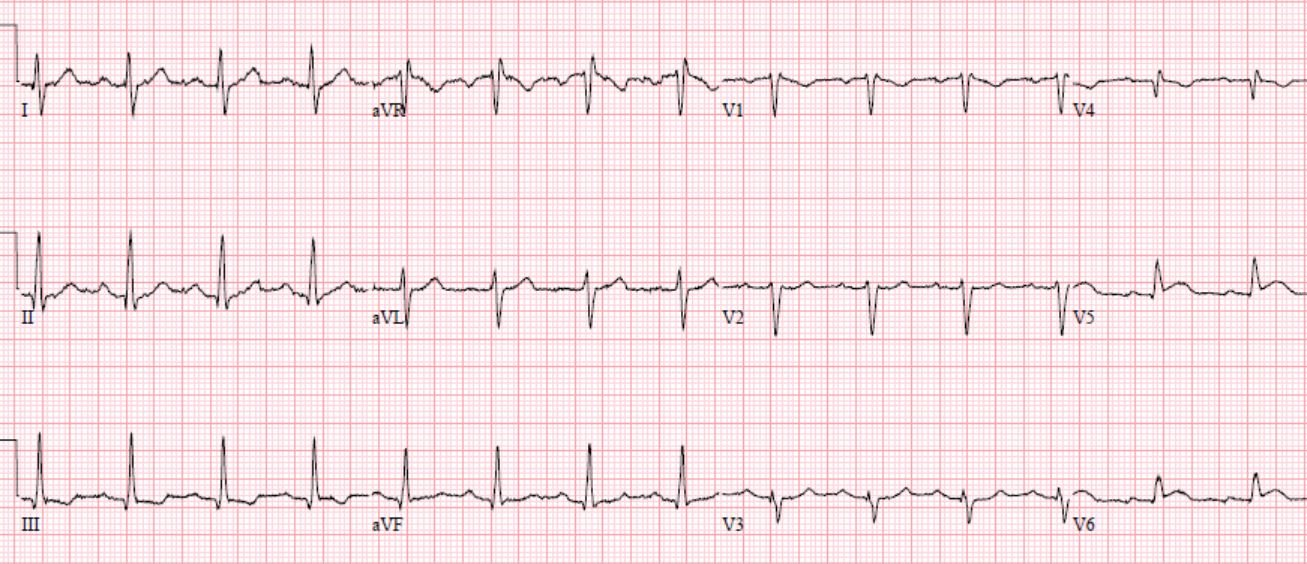
\includegraphics[width=\linewidth]{images/ecg_norm.jpg}
    \caption{Standard ECG Image.}
    \label{fig:ecgnorm}
  \end{subfigure}\hfill
  \begin{subfigure}[b]{0.35\linewidth}
    \centering
    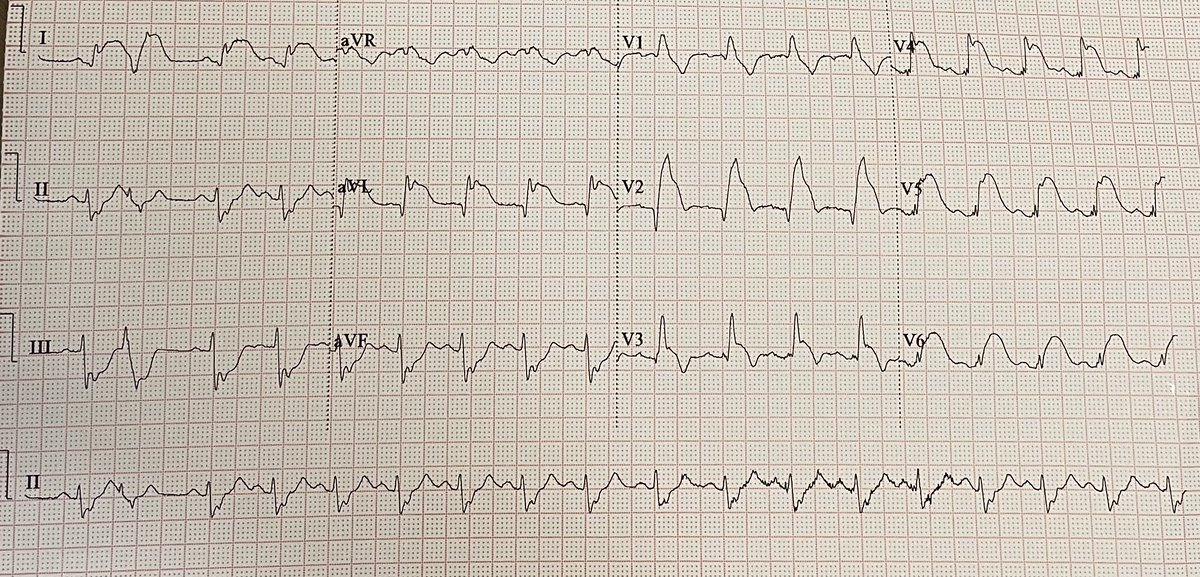
\includegraphics[width=\linewidth]{images/ecg_pict.jpg}
    \caption{ECG photographed (grid distorted).}
    \label{fig:ecgpict}
  \end{subfigure}\hfill
  \begin{subfigure}[b]{0.35\linewidth}
    \centering
    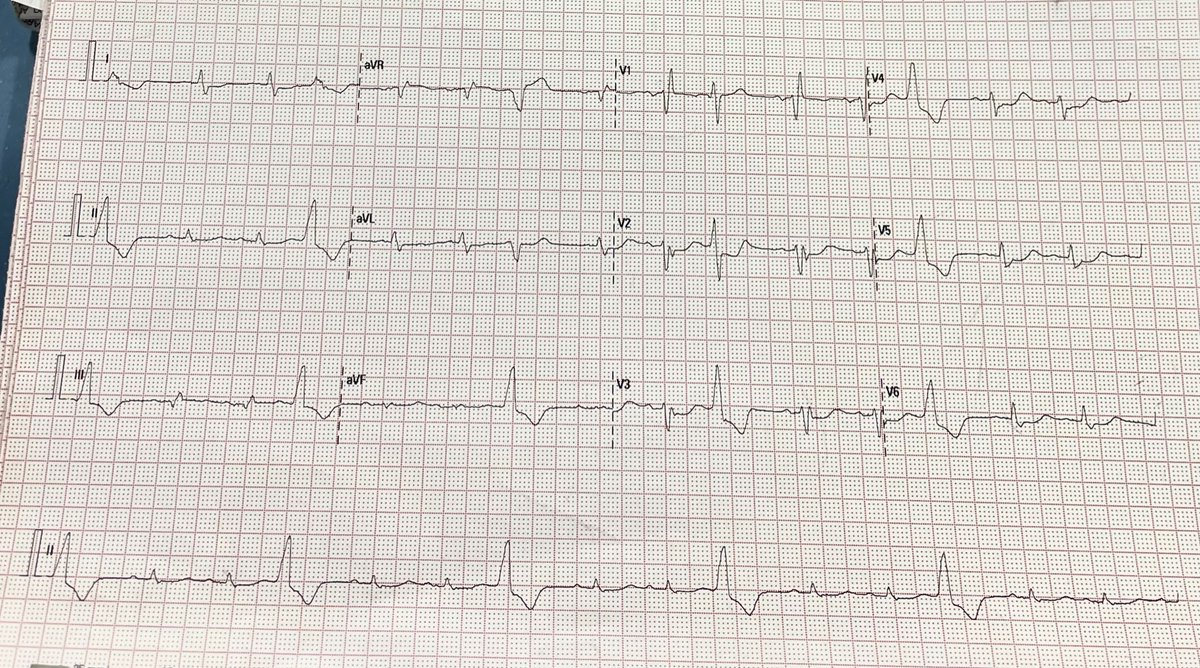
\includegraphics[width=\linewidth]{images/ecg_rotat.jpg}
    \caption{ECG photographed, with rotation.}
    \label{fig:ecgrotat}
  \end{subfigure}\hfill
  \begin{subfigure}[b]{0.35\linewidth}
    \centering
    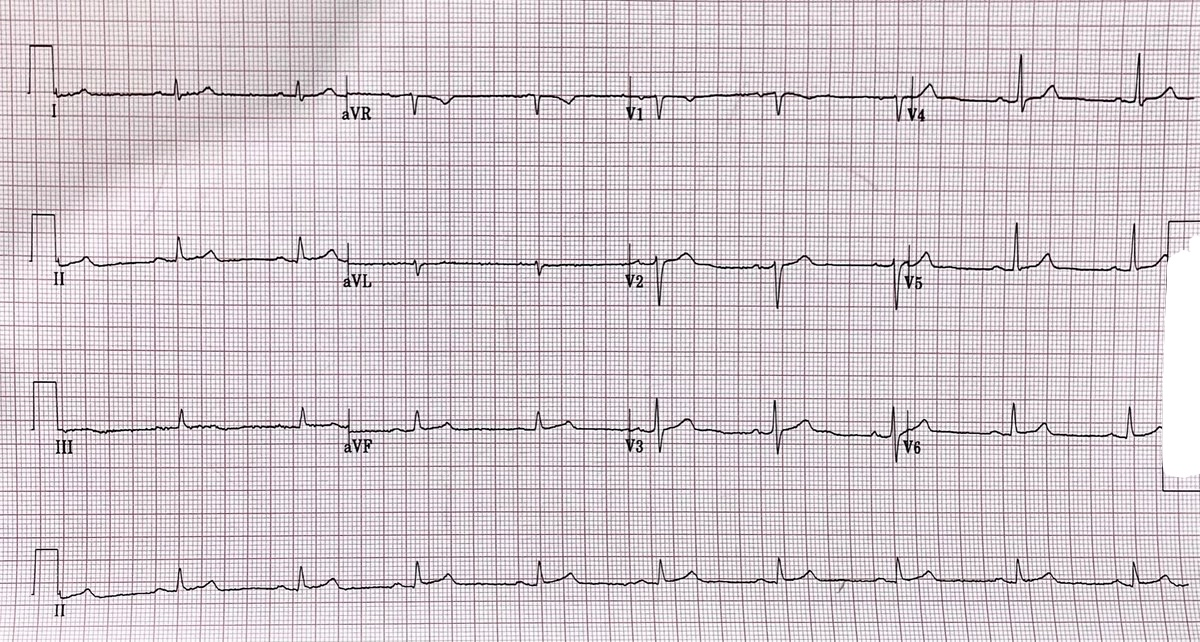
\includegraphics[width=\linewidth]{images/ecg_crease.jpg}
    \caption{ECG with a crease.}
    \label{fig:ecgcrease}
  \end{subfigure}\hfill
  \begin{subfigure}[b]{0.35\linewidth}
    \centering
    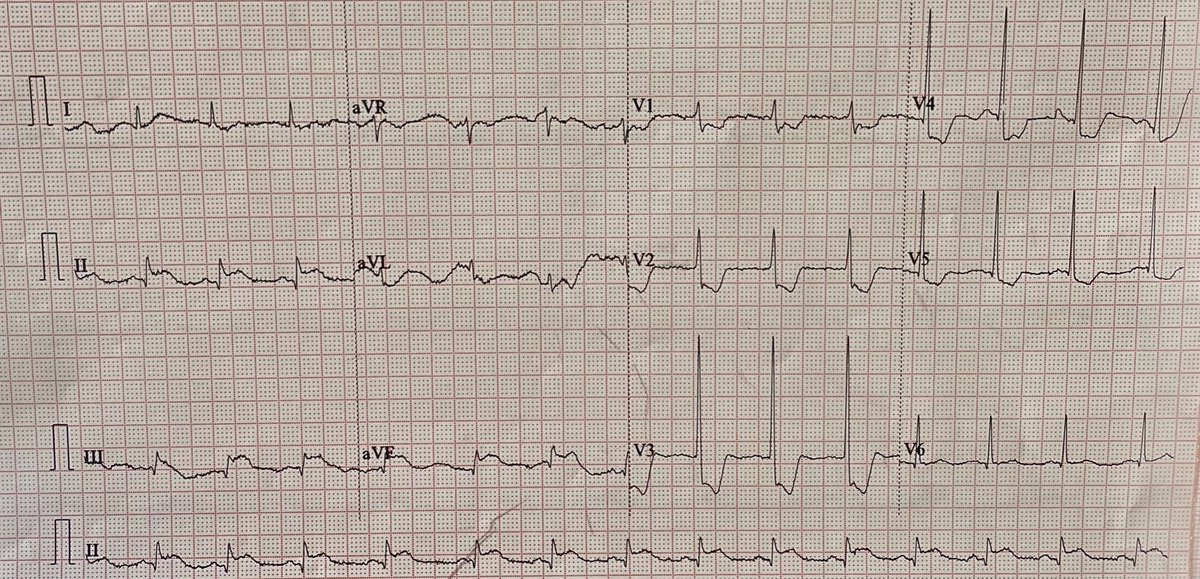
\includegraphics[width=\linewidth]{images/ecg_mark.jpg}
    \caption{ECG with pencil marks on them.}
    \label{fig:ecgmark}
  \end{subfigure}
  \caption{Various types of ECG images from the ECG-Image-Database.}
  \label{fig:ecgimages}
  \Description{Standard ECG Image.}
\end{figure}

% Glossary
\newpage
\section*{Glossary}
\addcontentsline{toc}{section}{Glossary} % CHANGED: toc level is "section" in the ACM template (no chapters)
\label{glossary}

\begingroup
\small
\renewcommand{\arraystretch}{1.5}
\begin{longtable}{@{}>{\raggedright\arraybackslash}p{0.27\linewidth} p{0.68\linewidth}@{}}
  \toprule
  \textbf{Term} & \textbf{Definition} \\
  \midrule
  \endfirsthead
  \toprule
  \textbf{Term} & \textbf{Definition} \\
  \midrule
  \endhead
  \bottomrule
  \endfoot
  \textbf{Arrhythmia} & Any abnormal heart rate or rhythm. \\
  \textbf{Atrial fibrillation (AFIB)} & An arrhythmia in which the atria beat irregularly, giving irregularly spaced beats without clear P waves. \\
  \textbf{Atrial flutter (AFLT)} & An arrhythmia with a rapid, regular atrial rhythm that appears as a saw-tooth pattern. \\
  \textbf{AUROC} & Area under the receiver operating characteristic curve: the probability that a classifier scores a random positive case above a random negative one. 0.5 is chance and 1.0 is perfect; it does not depend on a threshold. \\
  \textbf{Augmentation} & Artificially altering training images (for example adding blur, shadows or rotation) so the model learns to cope with real-world variation. \\
  \textbf{Bootstrap confidence interval} & A range for a metric found by repeatedly resampling the test set with replacement; used when classes are small. \\
  \textbf{Calibration} & How well a model's stated confidence matches how often it is correct; a calibrated 80\% prediction is right about 80\% of the time. \\
  \textbf{CLAHE} & Contrast-limited adaptive histogram equalisation: histogram equalisation applied to small regions, with a limit on contrast to avoid amplifying noise. \\
  \textbf{CNN} & Convolutional neural network: a neural network that learns small image filters, stacking layers to build up from edges to complex patterns. \\
  \textbf{Conduction disturbance (CD)} & An abnormality in how the electrical impulse travels through the heart, such as a bundle branch block. \\
  \textbf{Data leakage} & When information from the test set is present in training, making results look better than they would be on unseen data. \\
  \textbf{Domain adaptation} & Techniques that adapt a model trained on one kind of data (for example scans) to another (for example phone photographs). \\
  \textbf{ECE} & Expected calibration error: the weighted average gap between predicted confidence and observed frequency, over confidence bins. Lower is better. \\
  \textbf{ECG} & Electrocardiogram: a recording of the heart's electrical activity, taken from electrodes on the body surface. \\
  \textbf{ECG-Image-Database} & A public dataset of about 36,000 real images of printed ECGs (from PTB-XL and Emory Healthcare) that were degraded and then scanned or photographed. \\
  \textbf{ECG-Image-Kit} & A software tool that renders ECG signals into synthetic ECG images, optionally with artefacts. \\
  \textbf{Fold} & One of the fixed subsets a dataset is divided into; PTB-XL provides ten patient-wise folds for training, validation and testing. \\
  \textbf{FR / NFR} & Functional requirement (what the system does) / non-functional requirement (how well it does it). \\
  \textbf{Grad-CAM} & Gradient-weighted class activation mapping: a method that produces a heatmap of the image regions that most influenced a CNN's prediction for a class. \\
  \textbf{GUI} & Graphical user interface. \\
  \textbf{Heart rate (HR)} & Beats per minute, calculated from the RR interval as $60/\mathrm{RR}$. \\
  \textbf{Histogram equalisation (HE)} & Spreading an image's intensity values across the full range to increase contrast. \\
  \textbf{Hough transform} & A technique for detecting straight lines (such as grid lines or lead baselines) in an image. \\
  \textbf{Hypertrophy (HYP)} & Thickening of a heart chamber's wall, associated with changes in ECG amplitude. \\
  \textbf{Lead} & One of the twelve views of the heart's electrical activity recorded in a standard ECG. \\
  \textbf{MCC} & Matthews correlation coefficient: a single measure of classification quality, from $-1$ to $1$, that remains informative when classes are imbalanced. \\
  \textbf{MI} & Myocardial infarction (heart attack): damage to heart muscle from a loss of blood supply, often visible as ST-segment and T-wave changes. \\
  \textbf{MoSCoW} & A prioritisation method that rates requirements as Must, Should, Could or Won't have. \\
  \textbf{Multi-label classification} & Classification in which one input can belong to several classes at once, each with its own output. \\
  \textbf{Otsu thresholding} & A method that automatically chooses the intensity cut-off separating foreground from background. \\
  \textbf{P wave, QRS complex, T wave }& The deflections of one heartbeat: atrial activation, ventricular activation and ventricular recovery. \\
  \textbf{Pan--Tompkins algorithm} & A standard real-time algorithm for detecting QRS complexes in an ECG signal. \\
  \textbf{PLES} & Professional, legal, ethical and social issues. \\
  \textbf{PTB-XL} & A public dataset of 21,800 labelled twelve-lead ECG signals from about 19,000 patients. \\
  \textbf{RR interval} & The time between successive R peaks, used to measure heart rate and rhythm regularity. \\
  \textbf{RTM} & Requirements Traceability Matrix: a table mapping each requirement to its design element, deliverable, test case and result. \\
  \textbf{Sensitivity} & The share of true cases a classifier finds: $\mathrm{TP}/(\mathrm{TP}+\mathrm{FN})$. \\
  \textbf{Shortcut learning} & When a model relies on features that happen to correlate with the label in training data (such as printed text) instead of the features that matter. \\
  \textbf{Sinus bradycardia / tachycardia} & A normal rhythm that is slower than 60 / faster than 100 beats per minute. \\
  \textbf{SNR} & Signal-to-noise ratio: the strength of a signal relative to background noise, usually in decibels. \\
  \textbf{Specificity} & The share of non-cases a classifier correctly clears: $\mathrm{TN}/(\mathrm{TN}+\mathrm{FP})$. \\
  \textbf{ST/T change (STTC)} & Changes to the ST segment or T wave, often linked to ischaemia. \\
  \textbf{SUS} & System Usability Scale: a standard ten-item questionnaire giving a usability score from 0 to 100, where 68 is average. \\
  \textbf{Temperature scaling} & A calibration method that divides each class score by a single value $T$, fitted on validation data, before the sigmoid. \\
  \textbf{Transfer learning} & Starting from a network pretrained on another task (for example natural images) and fine-tuning it for the new task. \\
\end{longtable}
\endgroup
\section{Research Participant Questionnaire}
\label{app:questionnaire}
% CHANGED: the Microsoft Forms questionnaire, inserted as a PDF
The questionnaire below was delivered to participants through Microsoft Forms.

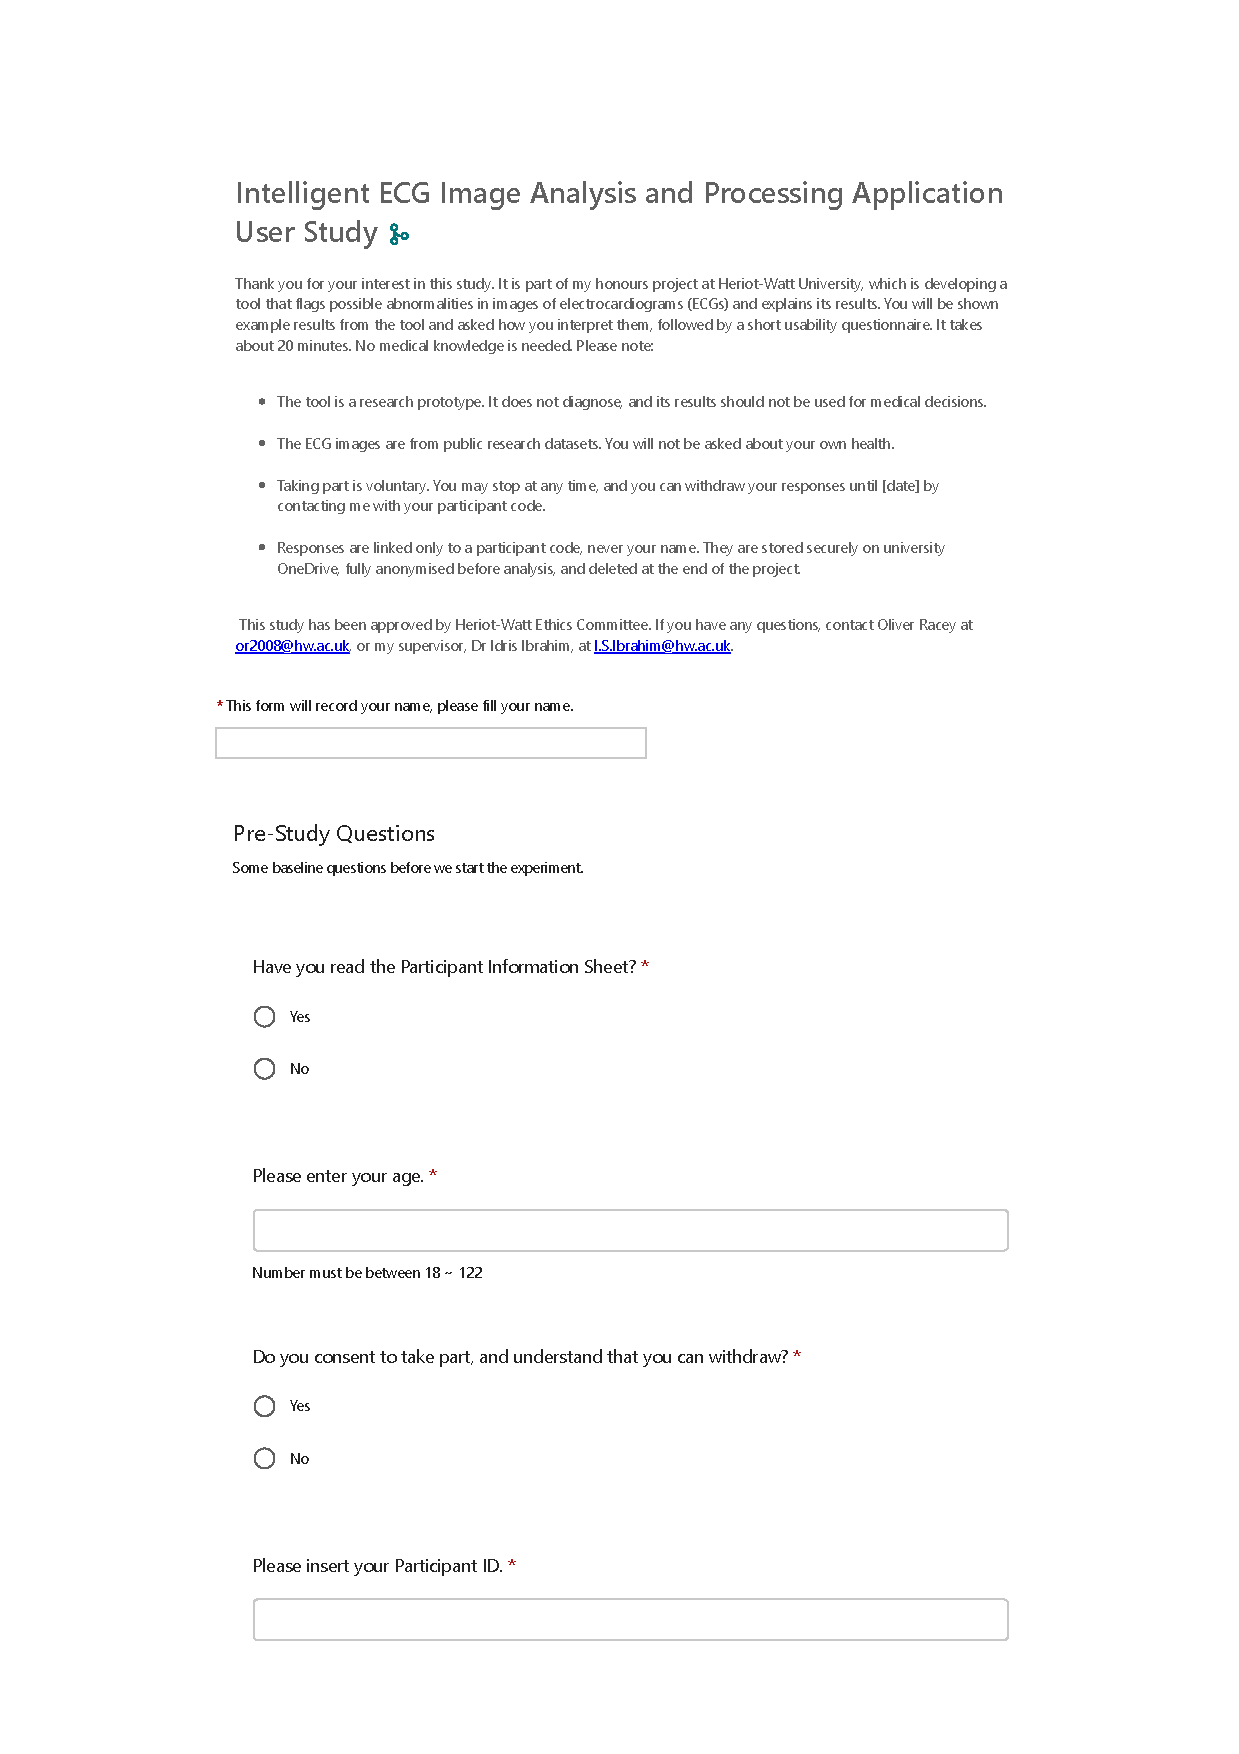
\includepdf[pages=-, scale=0.85, pagecommand={\thispagestyle{standardpagestyle}}]{images/IntelligentECGImageAnalysisAndProcessingApplicationUserStudy.pdf}
\end{document}